%%%%%%%%%%%%%%%%%%%%%%%%%%%%%%%%%%%%%%%%%%%%%%%%%%%%%%%%%%%%%%%%%%%%%%%
%
%   Presentation of Beamer AFRL 2018 Theme
%   Beamer Presentation by Emily Carper
%
%%%%%%%%%%%%%%%%%%%%%%%%%%%%%%%%%%%%%%%%%%%%%%%%%%%%%%%%%%%%%%%%%%%%%%%
\documentclass[t]{beamer}

\usetheme{AFRL2018}

\usepackage{lipsum}
\usepackage{tikz}
\usetikzlibrary{shapes,arrows}
\usetikzlibrary{decorations.pathreplacing}
\usepackage{hyperref}
\usepackage{smartdiagram}
\usepackage{metalogo}
\usepackage{graphicx}
\usepackage{multimedia}

\hypersetup{
    colorlinks=true,
    linkcolor=blue,
    filecolor=magenta,      
    urlcolor=cyan,
}
 
\urlstyle{same}

\title{AFRL Morph X}
%%\subtitle{A Software Licensing Opportunity}

\author{\large {Jeff Brown\\
  Alex Kaszynski}}

\institute{Engine Integrity Branch\\
  Turbine Engine Divsion\\
  Aerospace Systems Directorate}
    \date{\today}
    %%%%%      \vspace{5pt}xxxxxb
    % Turbine Engine Technology Symposium 2018}
\distribution{\small{\textbf{Distribution Statemeent A}}}
    %\distribution{\textbf{DISTRIBUTION STATEMENT C.} / Distribution authorized to U.S. Government Agencies and their contractors (Critical Technology) (Sep. 2018).  Other requests for this document shall be referred to AFRL/RQTI, 1950 Fifth Street, WPAFB, OH}
\conference{}
\begin{document}
\titleframe


%-------------------------------------------------------------------------------------------------------#
\frame{
  
  \frametitle{AFRL Morph X}
  \framesubtitle{3D Mesh Morphing Software}
\vspace{-5mm}
\begin{columns}
  \begin{column}{0.6\textwidth}

  \begin{itemize}
  \item Move 3D FEM and CFD meshes to point cloud and surface data
  \item Save design time by removing mesh generation bottlenecks
  \item Rapidly assess impacts of as-manufactured geometry on design intent
  \item Learn the effects of operational damage on continued operation
  \item Design and validate the suitability of component repair
  \item And more...
  
  \end{itemize}

  \end{column}
  \begin{column}{0.4\textwidth}
    \vspace{7mm}
    %% \smartdiagramset{font=\small,
    %% distance planet-satellite=3cm}
    %% \scalebox{0.6}{\smartdiagram[connected constellation diagram]{AFRL Morph X,
    %%     Design, Repair, Operation, Manufacture}}
    \smartdiagramset{font=\small}
    \scalebox{0.55}{\smartdiagram[bubble diagram]{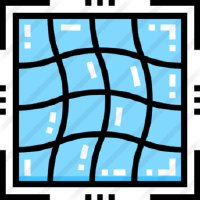
\includegraphics[height=2.0cm]{./figures/morph_logo.png} \\AFRL Morph\\ X,
        Design, Repair, Operation, Manufacture}}
    
  \end{column}
\end{columns}
  
}
%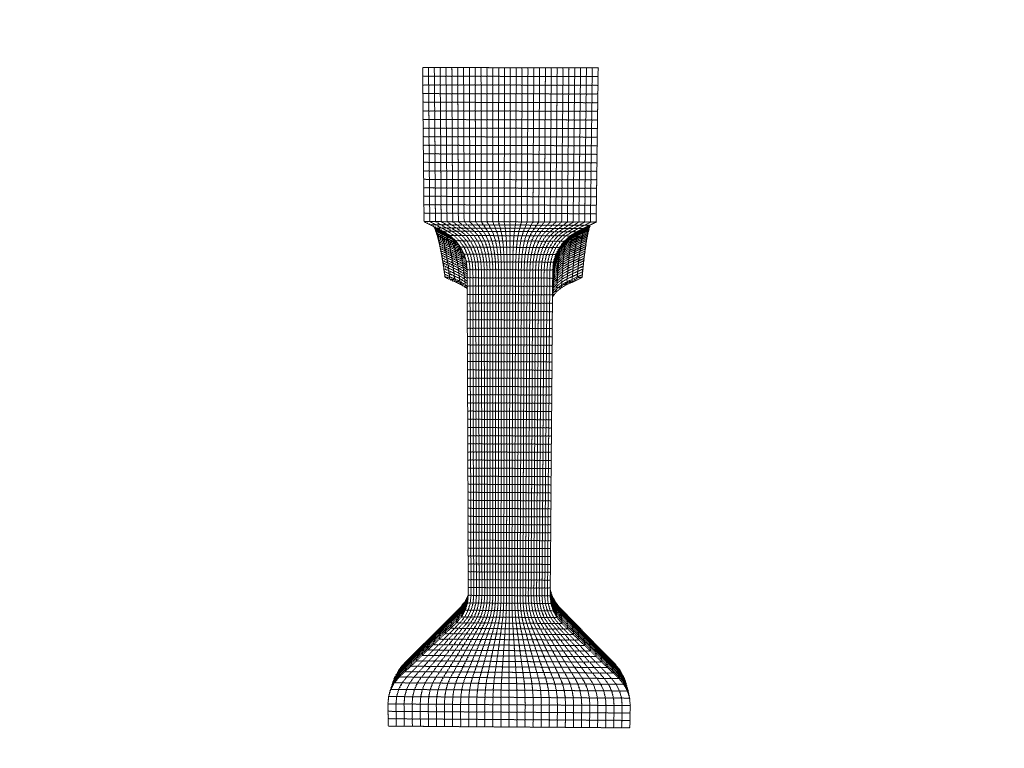
\includegraphics[height=1.0]{./figures/diskfem_side.png}

%-------------------------------------------------------------------------------------------------------#
\begin{frame}
  \frametitle{Design with AFRL Morph X}
  \framesubtitle{Update FEM to Parametrically Variable CAD Surface}
  \begin{center}

    \vspace{-11mm}

\begin{center}
    \begin{tikzpicture}
      % trim (left, lower, right uppert)
      \node (img1) {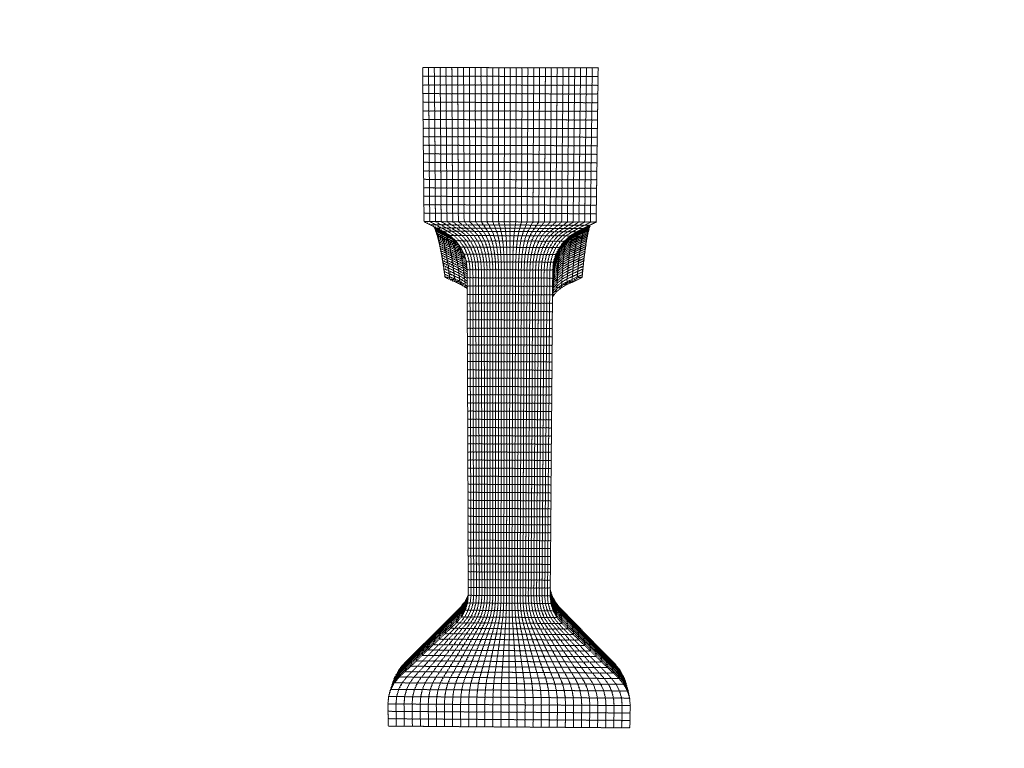
\includegraphics[height=4.5cm, trim={14cm, 0cm, 0cm, 0cm}, clip]{./figures/diskfem_side.png}};
      \node (img2) at (img1.east) [yshift=0.0cm]{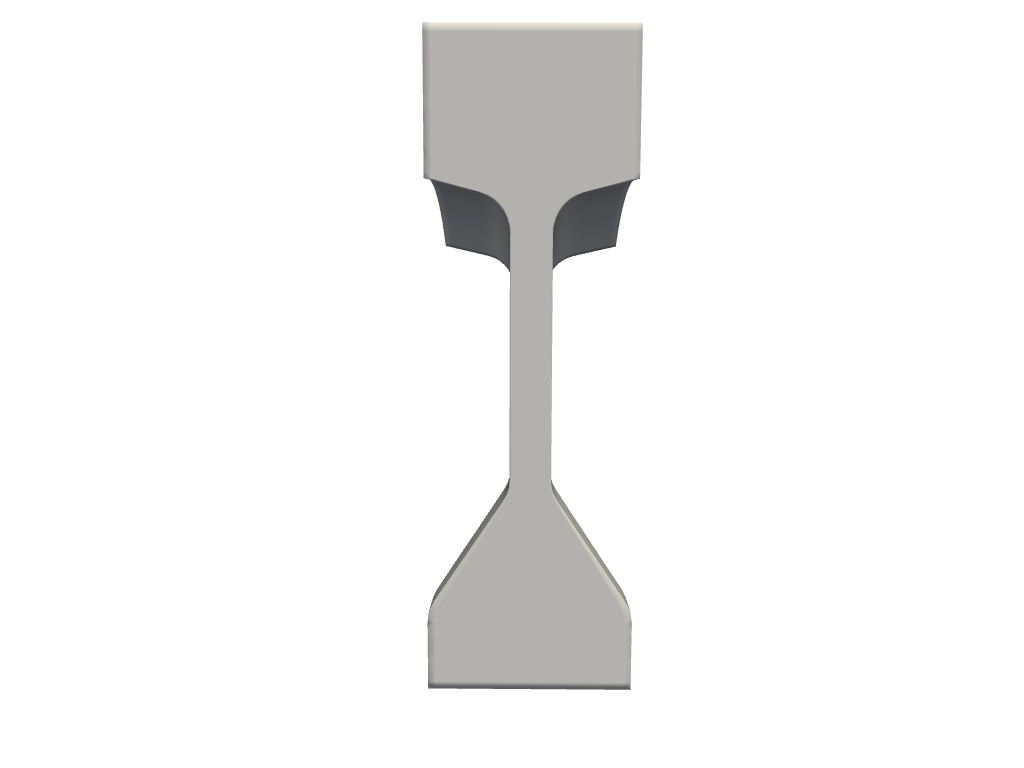
\includegraphics[height=4.5cm, trim={7cm, 0cm, 0cm, 0cm}, clip]{./figures/diskcad_side.png}};
      \node (img3) at (img2.east) [xshift=1.0cm, yshift=0.1cm]{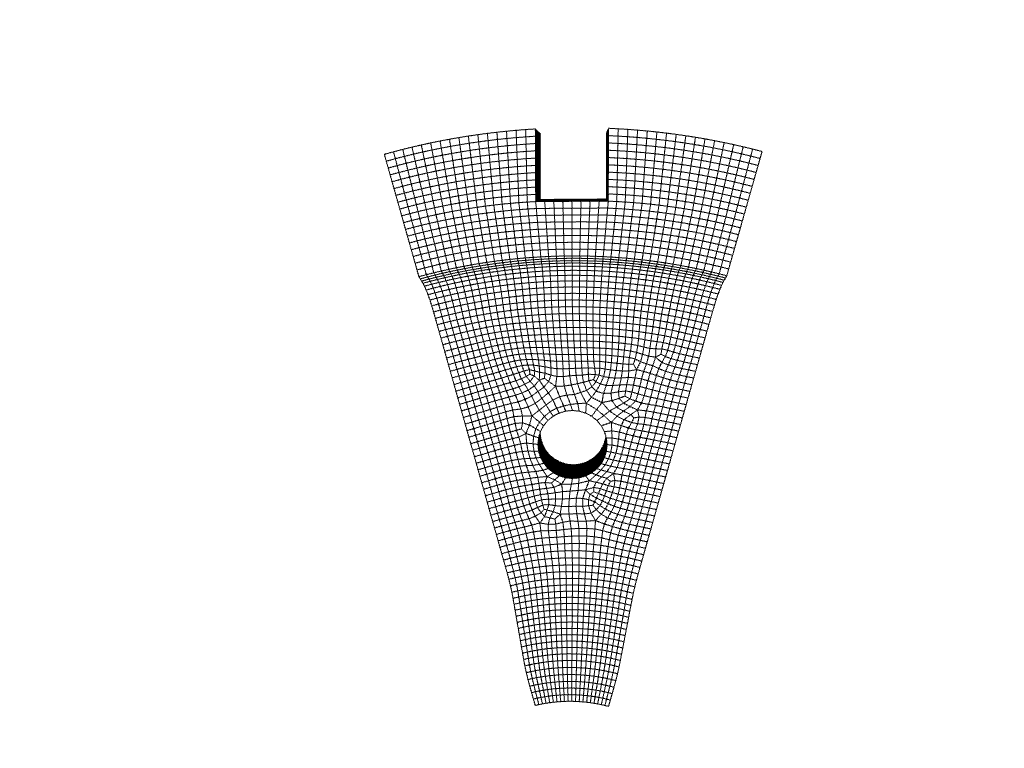
\includegraphics[height=4.9cm, trim={13.0cm, 0cm, 3cm, 1cm}, clip]{./figures/diskfem_front.png}};
      \node (img4) at (img3.east) [xshift=0.25cm, yshift=0.1cm]{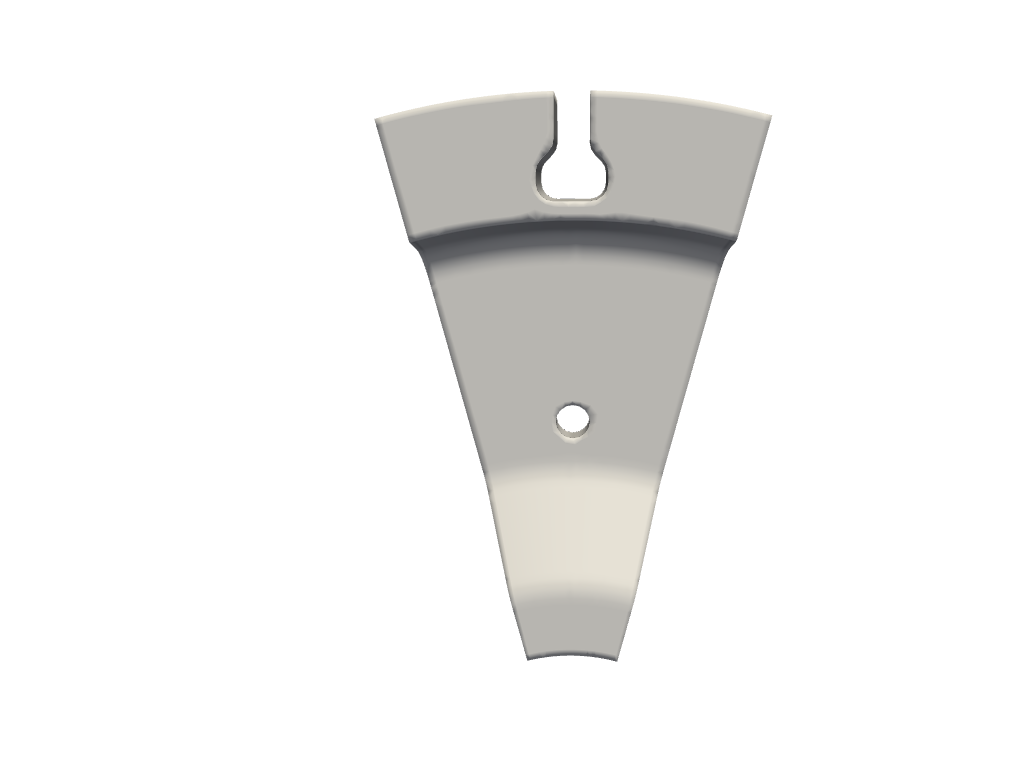
\includegraphics[height=4.9cm, trim={13cm, 0cm, 9cm, 1cm}, clip]{./figures/diskcad_front.png}};

      \node [] at (-1.25, -2.5) (cap1) [align=center]{FEM};
      \node [] at (1.5, -2.5) (cap2) [align=center]{Target CAD};
      \node [] at (4.85, -2.5) (cap3) [align=center]{FEM};
      \node [] at (7.75, -2.5) (cap4) [align=center]{Target CAD};

      \node [] at (0, -3.15) (cap5) [align=center, font=\bfseries]{Side View};
      \node [] at (6.25, -3.15) (cap6) [align=center, font=\bfseries]{Front View};

      \node [draw] at (3.55, -4.0) (cap7) [align=center]{\footnotesize Models plotted in same reference frame.  FEM grows radially.\\Fourteen variable geometry parameters.};

      %\node [draw] at (3.55, -3.5) (cap7) [align=center]{\footnotesize Bore Radius, Bore Width, Bore height, Web Height, Web Thickness, Rim Radius,\\ \footnotesize Bolt Hole Radius, Bolt Hole Diameter, 6x Dovetail Parameters};


      
    \end{tikzpicture}
\end{center}


  \end{center}    
\end{frame}

%-------------------------------------------------------------------------------------------------------#
\begin{frame}
  \frametitle{Design with AFRL Morph X}
  \framesubtitle{Update FEM to Parametrically Variable CAD Surface}
  \begin{center}

    \vspace{-5mm}

    \begin{tikzpicture}
      % trim (left, lower, right uppert)
      \node (img1) {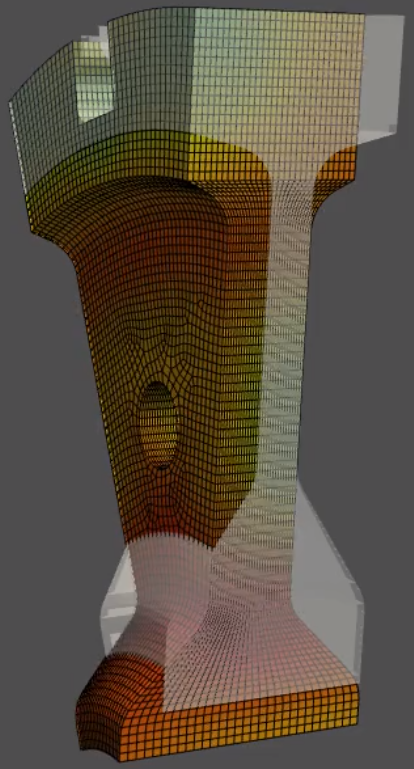
\includegraphics[height=3.0cm]{./figures/disk_side_1.png}};
      \node (img2) at (img1.south east) [xshift=1.0cm]{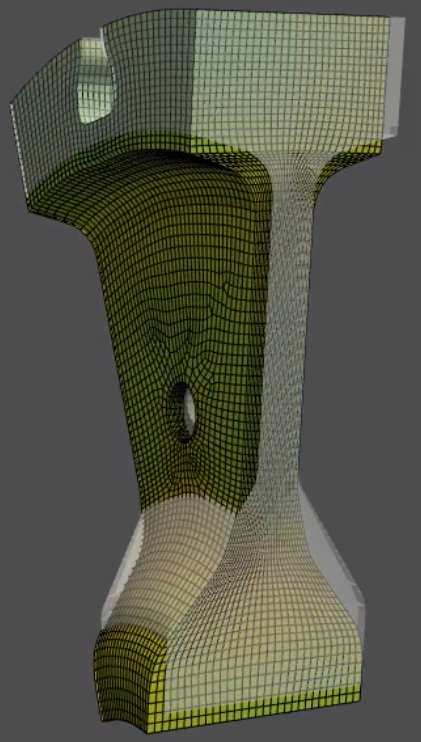
\includegraphics[height=3.0cm]{./figures/disk_side_2.png}};
      \node (img3) at (img2.south east) [xshift=1.0cm]{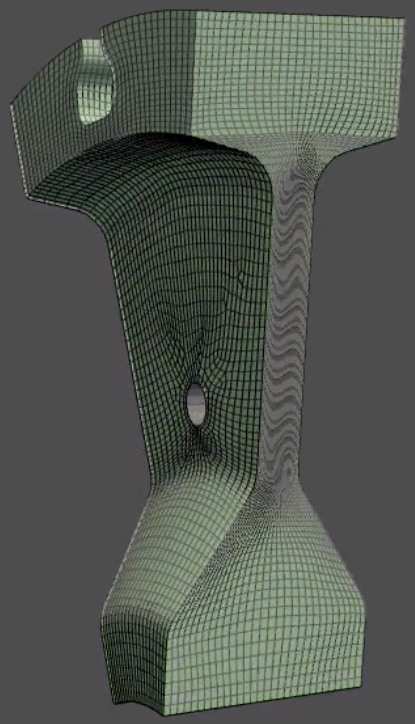
\includegraphics[height=3.0cm]{./figures/disk_side_3.png}};

      \node (img4) at (img1.east) [xshift=4.0cm]{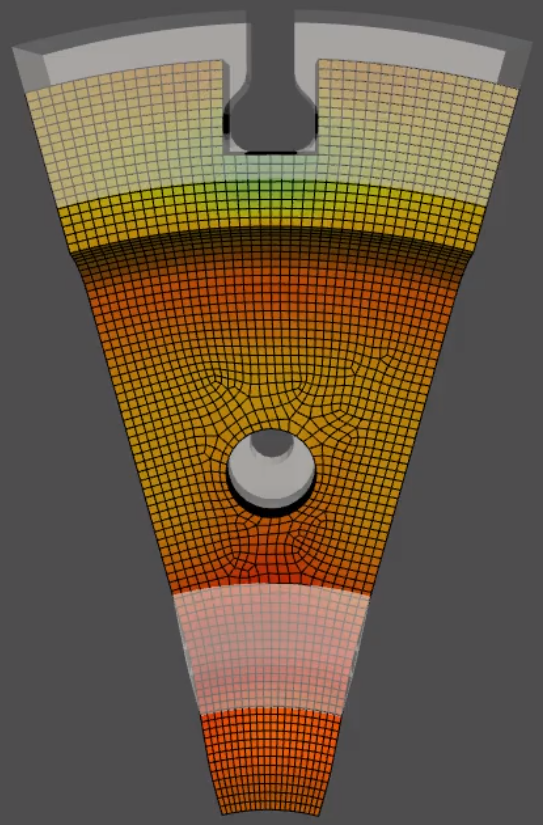
\includegraphics[height=3.0cm]{./figures/disk_front_1.png}};
      \node (img5) at (img4.south east) [xshift=1.0cm, yshift=0.1cm]{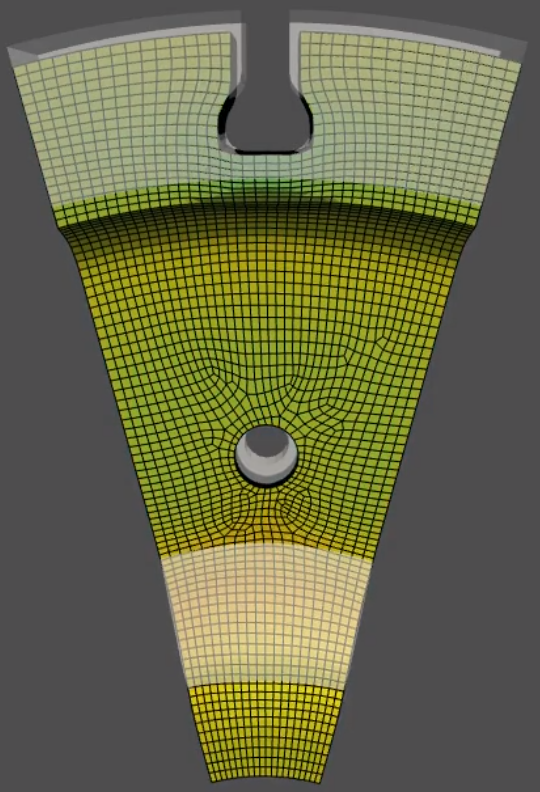
\includegraphics[height=3.0cm]{./figures/disk_front_2.png}};
      \node (img6) at (img5.south east) [xshift=1.0cm]{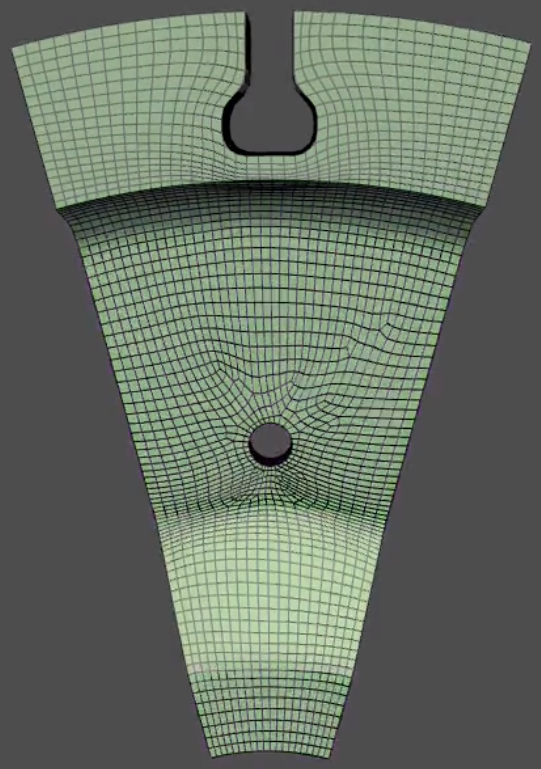
\includegraphics[height=3.0cm]{./figures/disk_front_3.png}};
      
    \end{tikzpicture}
       
\end{center}    
\end{frame}
%-------------------------------------------------------------------------------------------------------#
\begin{frame}
  \frametitle{Animation - Click image to Play}
  %%\framesubtitle{Morph Simple Plate FEM to Complex 3D Turbine Airfoil Surface}

  \begin{figure}
    \centering    
    \movie[label=show4, width=0.75\textwidth, poster, autostart, showcontrols, loop]{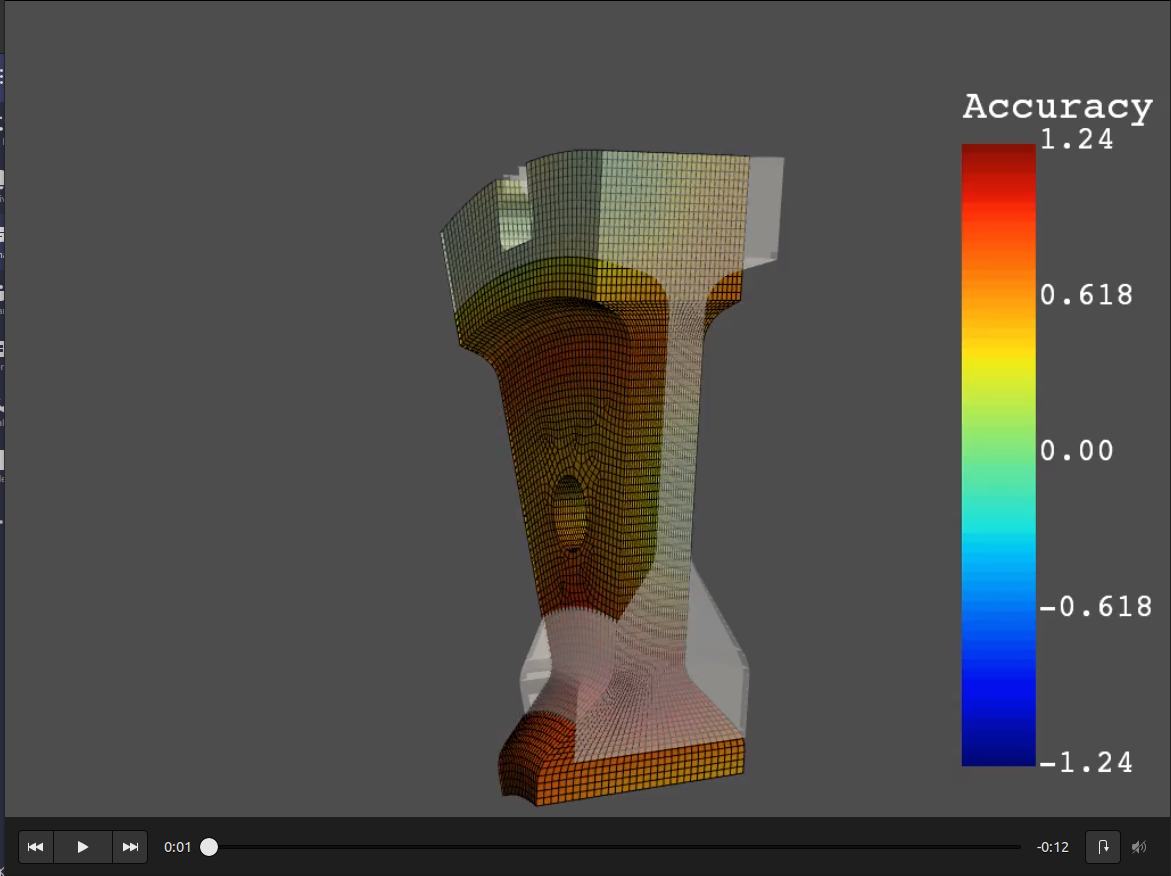
\includegraphics[width=0.75\textwidth]{./figures/diskside_cover.png}}{./figures/disk_side.mp4}
 \end{figure} 
\end{frame}

%-------------------------------------------------------------------------------------------------------#
\begin{frame}
  \frametitle{Animation - Click image to Play}
  %%\framesubtitle{Morph Simple Plate FEM to Complex 3D Turbine Airfoil Surface}

  \begin{figure}
    \centering    
    \movie[label=show4, width=0.75\textwidth, poster, autostart, showcontrols, loop]{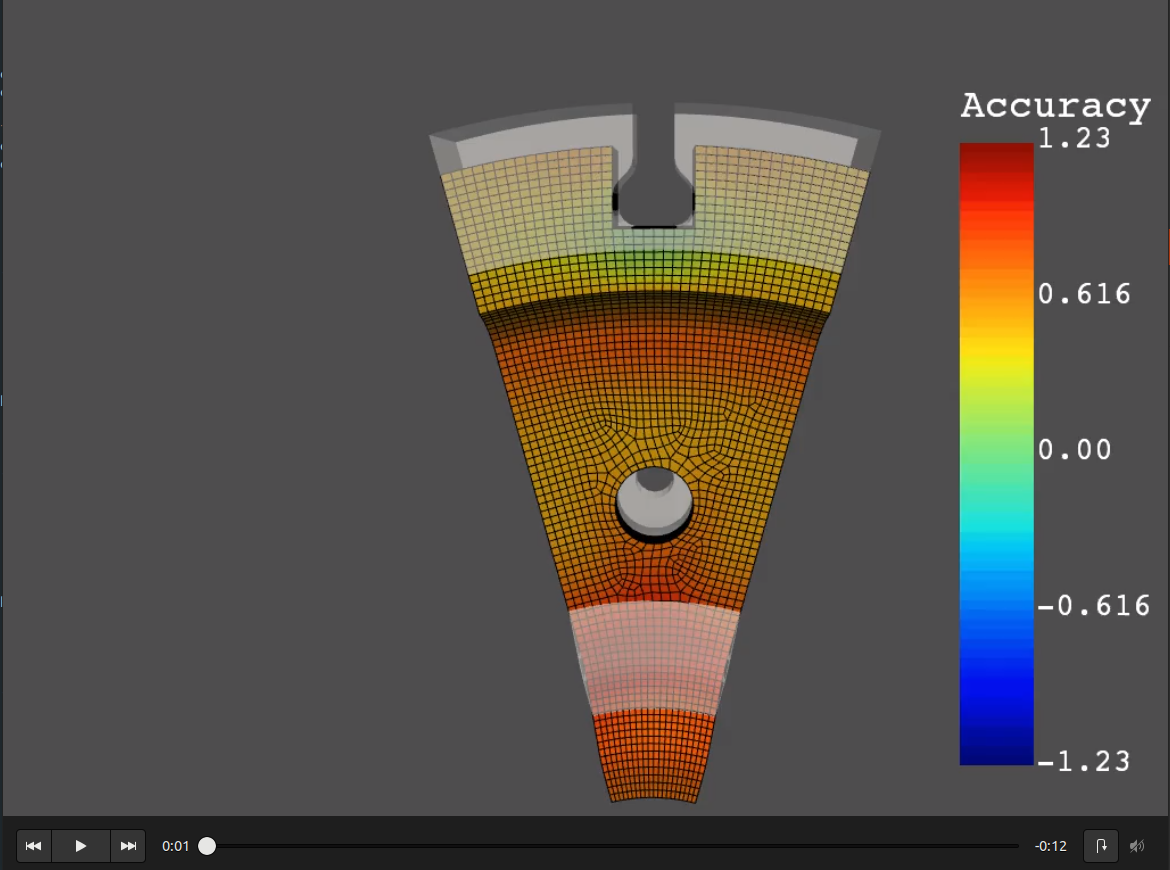
\includegraphics[width=0.75\textwidth]{./figures/diskfront_cover.png}}{./figures/disk_front.mp4}
 \end{figure} 
\end{frame}

%-------------------------------------------------------------------------------------------------------#
\begin{frame}
  \frametitle{Design with AFRL Morph X}
  \framesubtitle{Sample Large Design Spaces Without Remeshing Challenges}

  \tikzstyle{decision} = [diamond, draw, fill=blue!20, 
    text width=4.5em, text badly centered, node distance=3cm, inner sep=0pt]
  \tikzstyle{block} = [rectangle, draw, fill=white!20, 
    text width=4em, text centered, rounded corners, minimum height=1em, inner sep=0.025cm]

  \tikzstyle{line} = [draw, -latex']
  \tikzstyle{cloud} = [draw, ellipse,fill=red!20, node distance=3cm,7
    minimum height=2em]
  
  \begin{tikzpicture}

    %\node (circle) [circle] at (-1.35, -0.05) [align=center, yshift=-0.75cm, xshift=1.5cm, color=white, fill=blue, inner sep=2pt]{AFRL\\ MORPH X};
    \node [draw] at (0.15, -0.80) (logo) {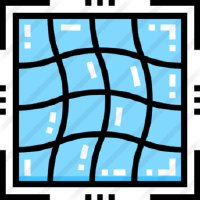
\includegraphics[height=1.75cm]{./figures/morph_logo.png}};%{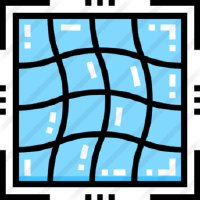
\includegraphics{./figures/morph_logo.png}};
    \node [] at (0.15, -2.25) (caption) [align=center]{AFRL\\MORPH X};%{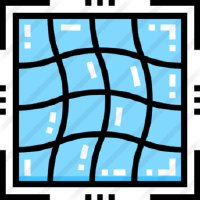
\includegraphics{./figures/morph_logo.png}};
    \node [draw] at (0.1, 1) (cad) [align=center, fill=blue!20]{Parametric\\ CAD};
    \node [] at (0.1, 2.25) (doe) [align=center]{Airfoil Blend\\ DoE Matrix};
    \draw [->] (0.1, 0.5) -- (0.1, 0.2);
    \draw [->] (0.1, 1.85) -- (0.1, 1.5);

    \draw [->] [color=blue, line width=0.45mm] (1.1, -0.75) -- (2.0, -0.75);
    
    
    \node [block, right of=logo, xshift=1.8cm, yshift=0.8cm] (block1) {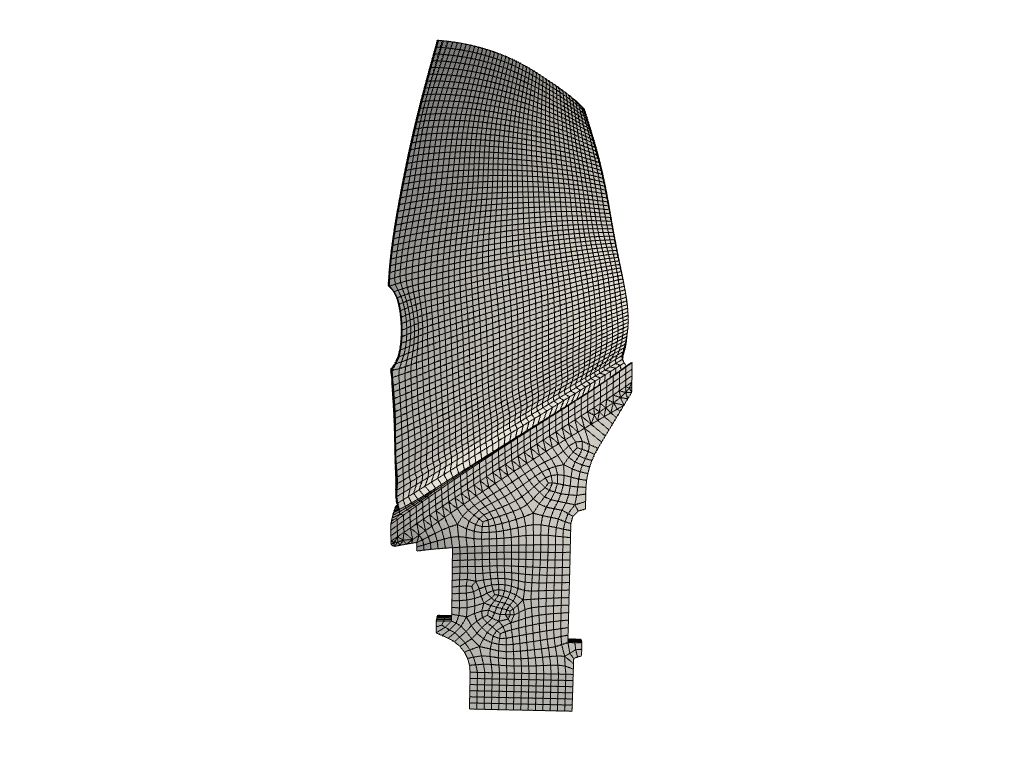
\includegraphics[height=1.0cm, , trim={13cm, 7cm, 13cm, 1cm}, clip]{./figures/pbs4_blend_1.png}};
    \node [block, right of=block1, xshift=1.0cm] (block2) {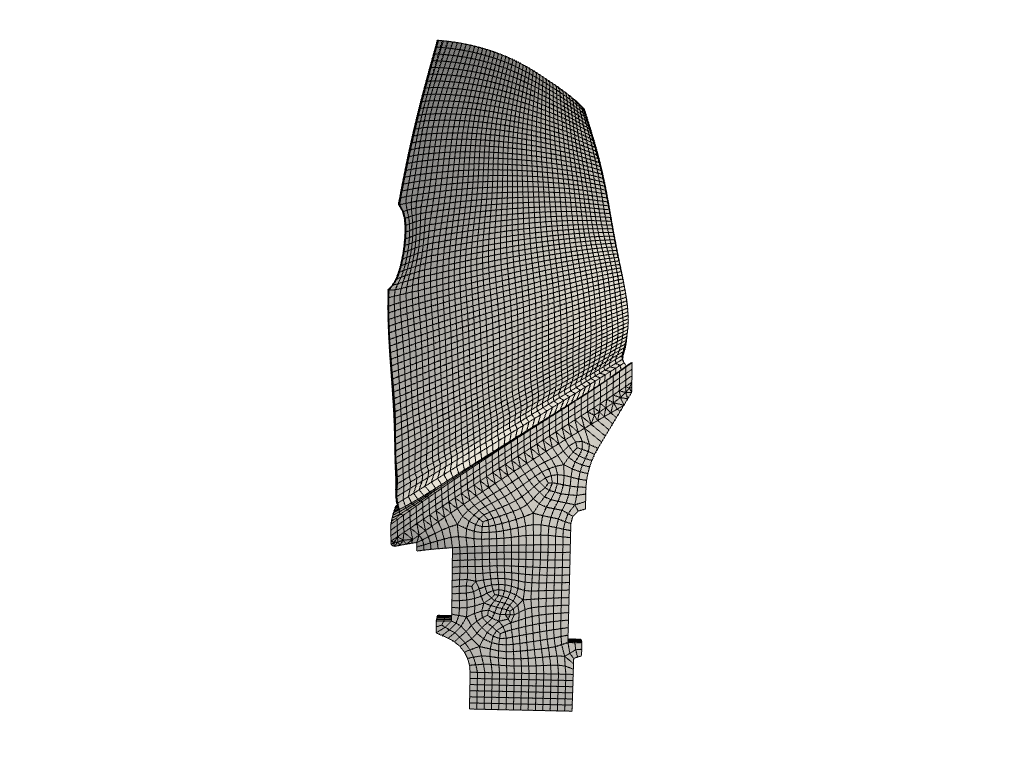
\includegraphics[height=1.0cm, , trim={13cm, 7cm, 13cm, 1cm}, clip]{./figures/pbs4_blend_2.png}};
    \node [block, right of=block2, xshift=1.0cm] (block3) {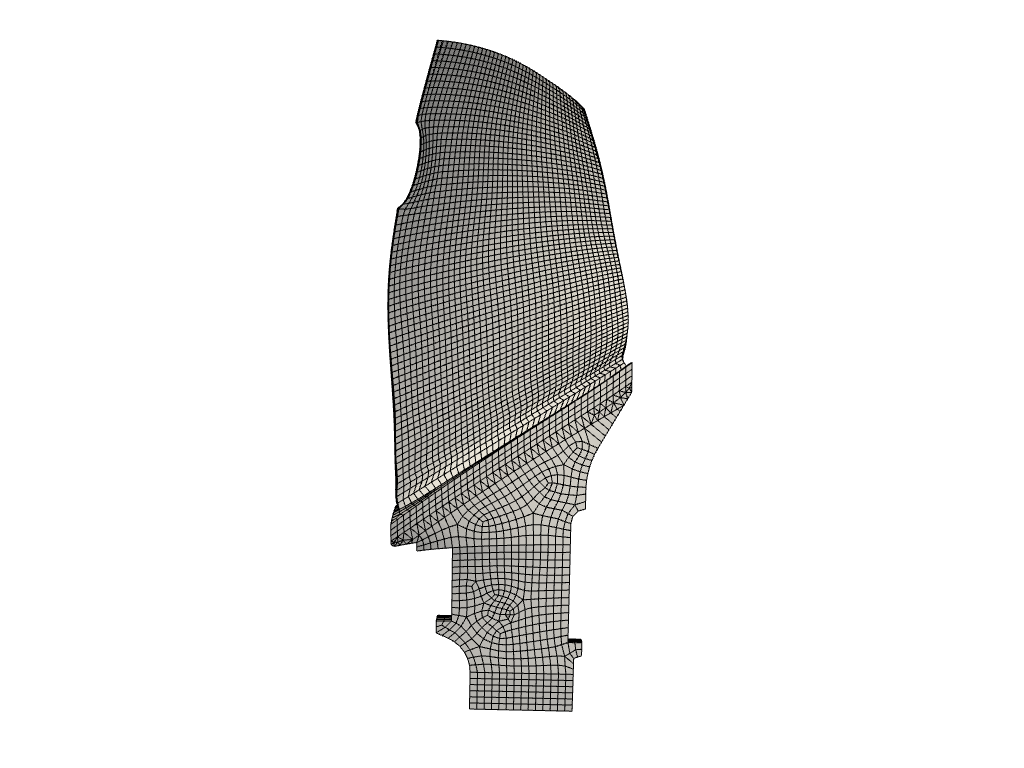
\includegraphics[height=1.0cm, , trim={13cm, 7cm, 13cm, 1cm}, clip]{./figures/pbs4_blend_3.png}};
    \node [block, right of=block3, xshift=1.0cm] (block4) {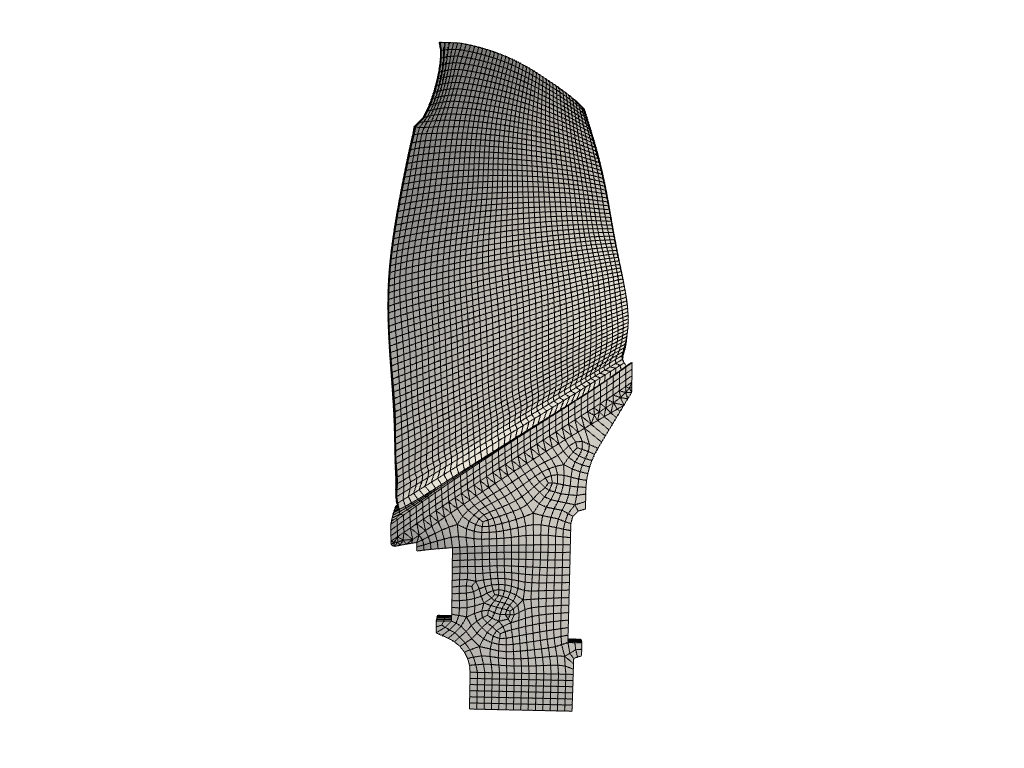
\includegraphics[height=1.0cm, , trim={13cm, 7cm, 13cm, 1cm}, clip]{./figures/pbs4_blend_4.png}};
    
    \node [block, above of=block1, yshift=0.1cm] (block5) {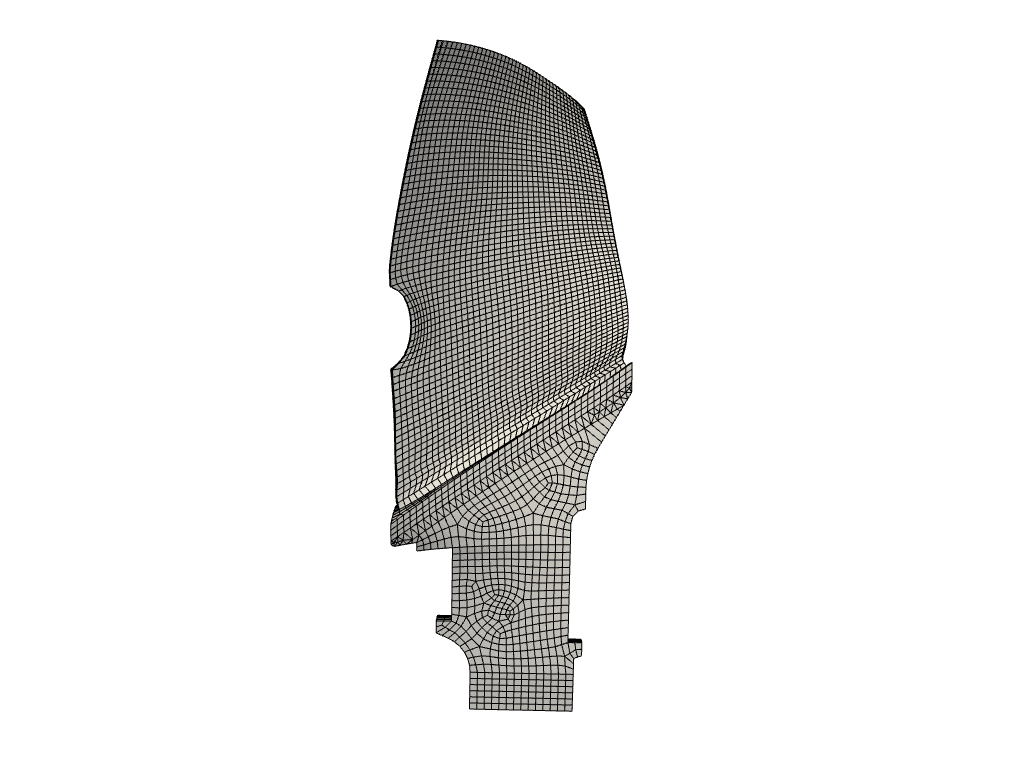
\includegraphics[height=1.0cm, , trim={13cm, 7cm, 13cm, 1cm}, clip]{./figures/pbs4_blend_5.png}};
    \node [block, above of=block2, yshift=0.1cm] (block6) {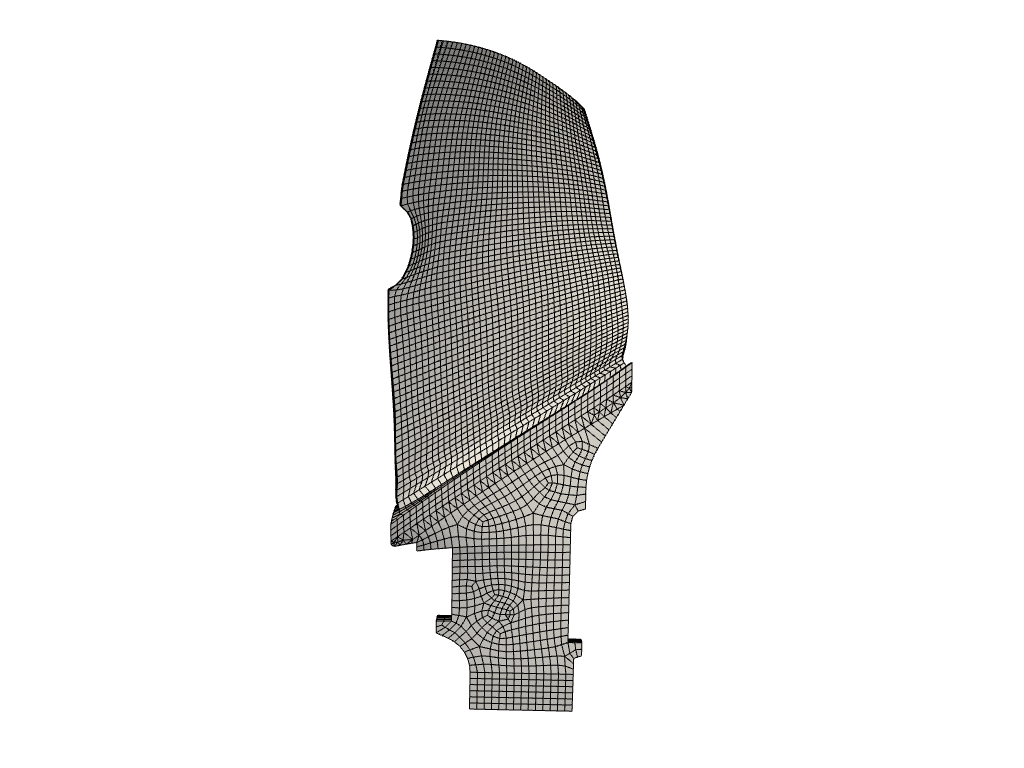
\includegraphics[height=1.0cm, , trim={13cm, 7cm, 13cm, 1cm}, clip]{./figures/pbs4_blend_6.png}};
    \node [block, above of=block3, yshift=0.1cm] (block7) {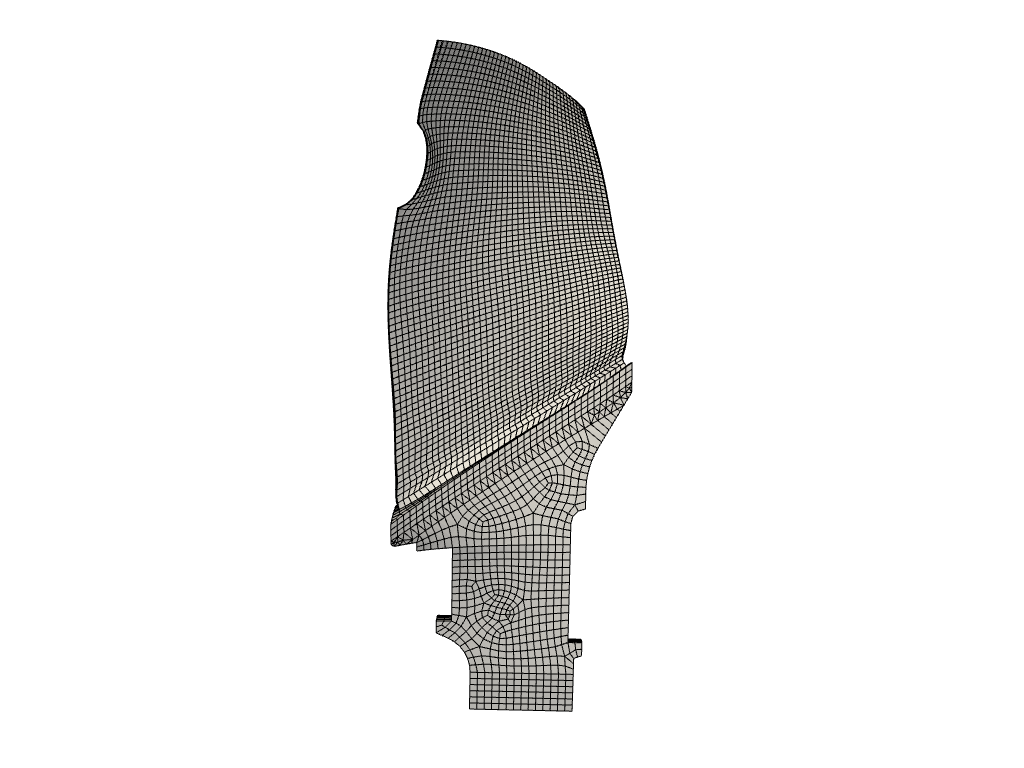
\includegraphics[height=1.0cm, , trim={13cm, 7cm, 13cm, 1cm}, clip]{./figures/pbs4_blend_7.png}};
    \node [block, above of=block4, yshift=0.1cm] (block8) {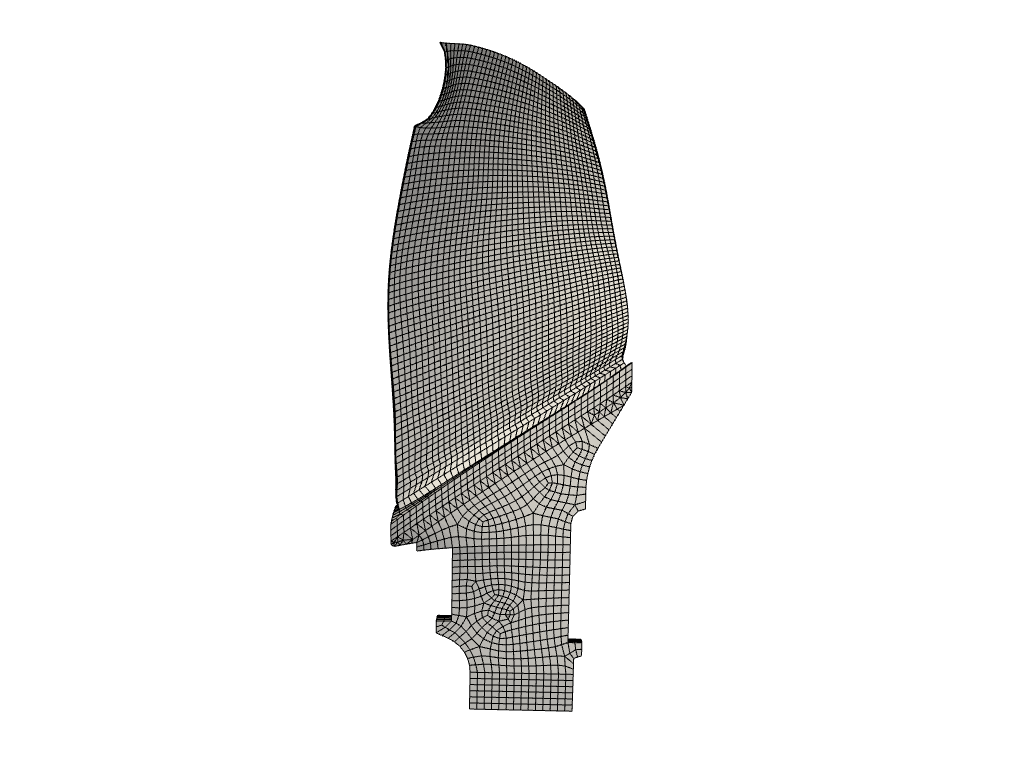
\includegraphics[height=1.0cm, , trim={13cm, 7cm, 13cm, 1cm}, clip]{./figures/pbs4_blend_8.png}};

    \node [block, above of=block5, yshift=0.1cm] (block9) {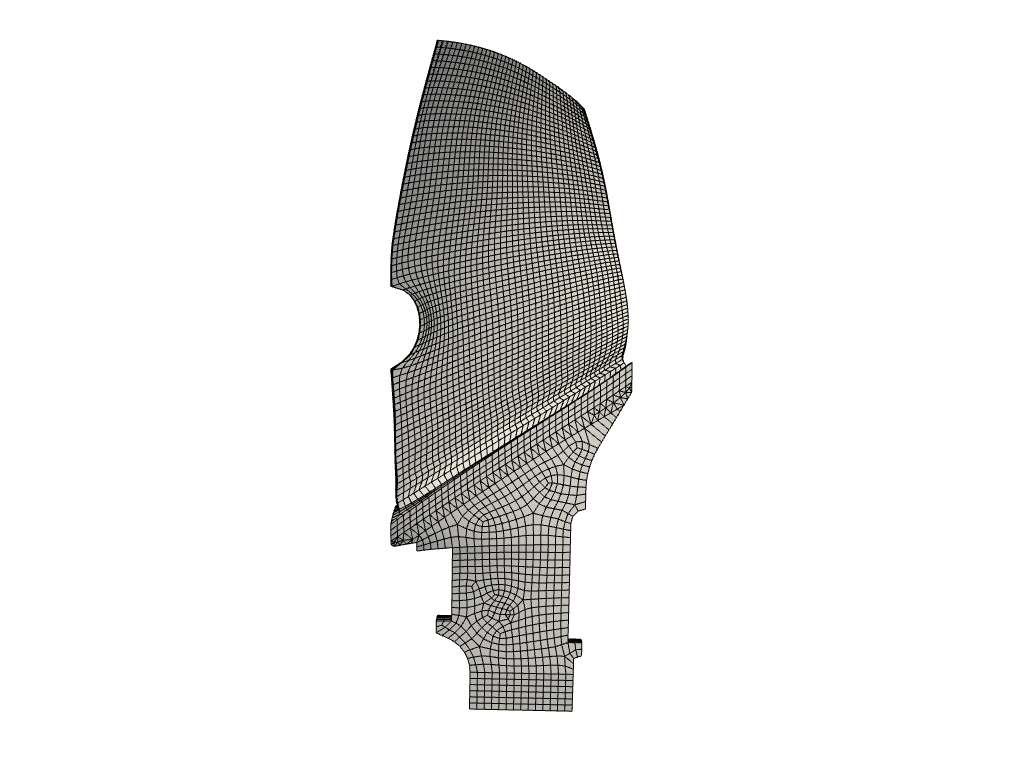
\includegraphics[height=1.0cm, , trim={13cm, 7cm, 13cm, 1cm}, clip]{./figures/pbs4_blend_9.png}};
    \node [block, above of=block6, yshift=0.1cm] (block10) {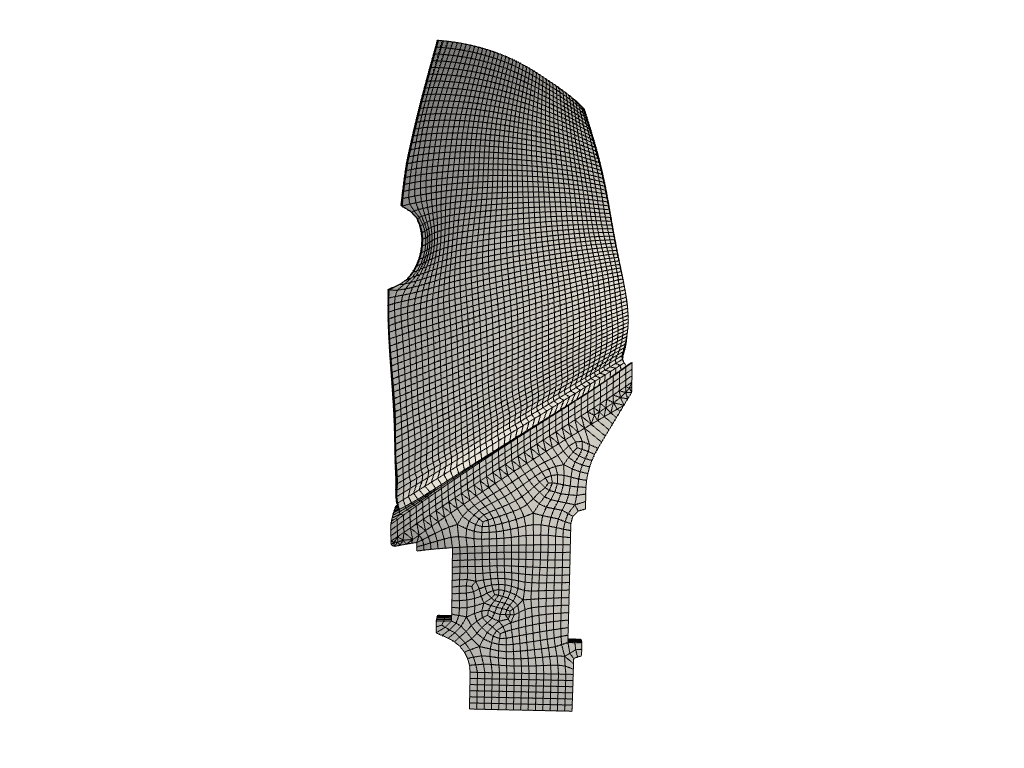
\includegraphics[height=1.0cm, , trim={13cm, 7cm, 13cm, 1cm}, clip]{./figures/pbs4_blend_10.png}};
    \node [block, above of=block7, yshift=0.1cm] (block11) {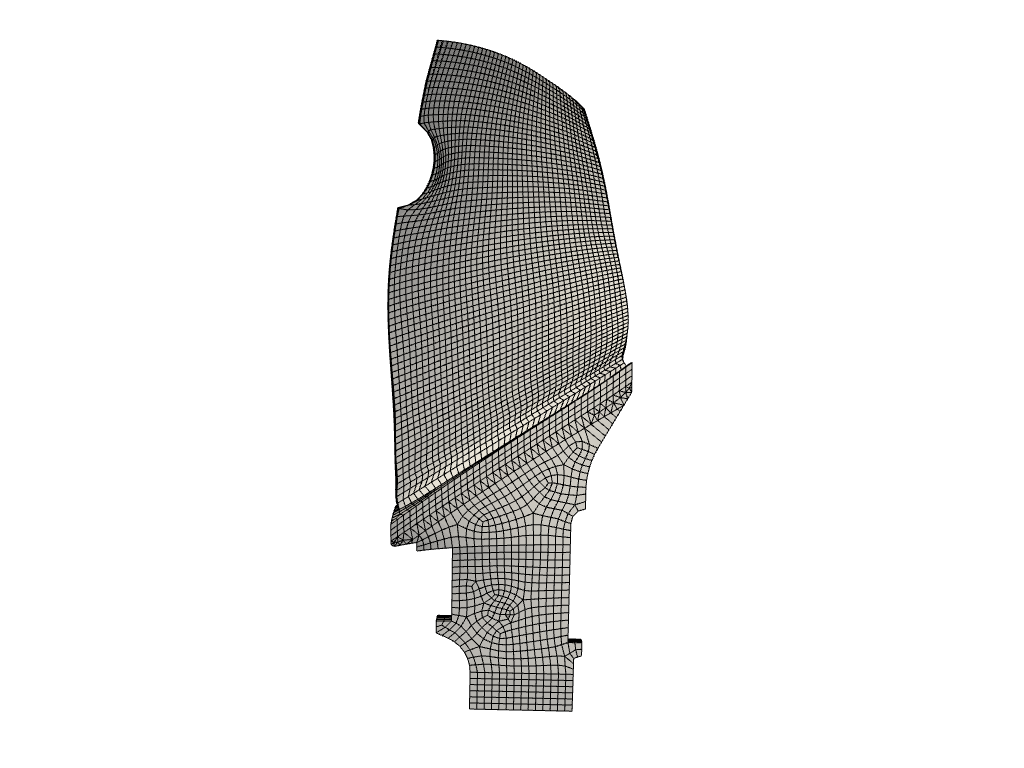
\includegraphics[height=1.0cm, , trim={13cm, 7cm, 13cm, 1cm}, clip]{./figures/pbs4_blend_11.png}};
    \node [block, above of=block8, yshift=0.1cm] (block12) {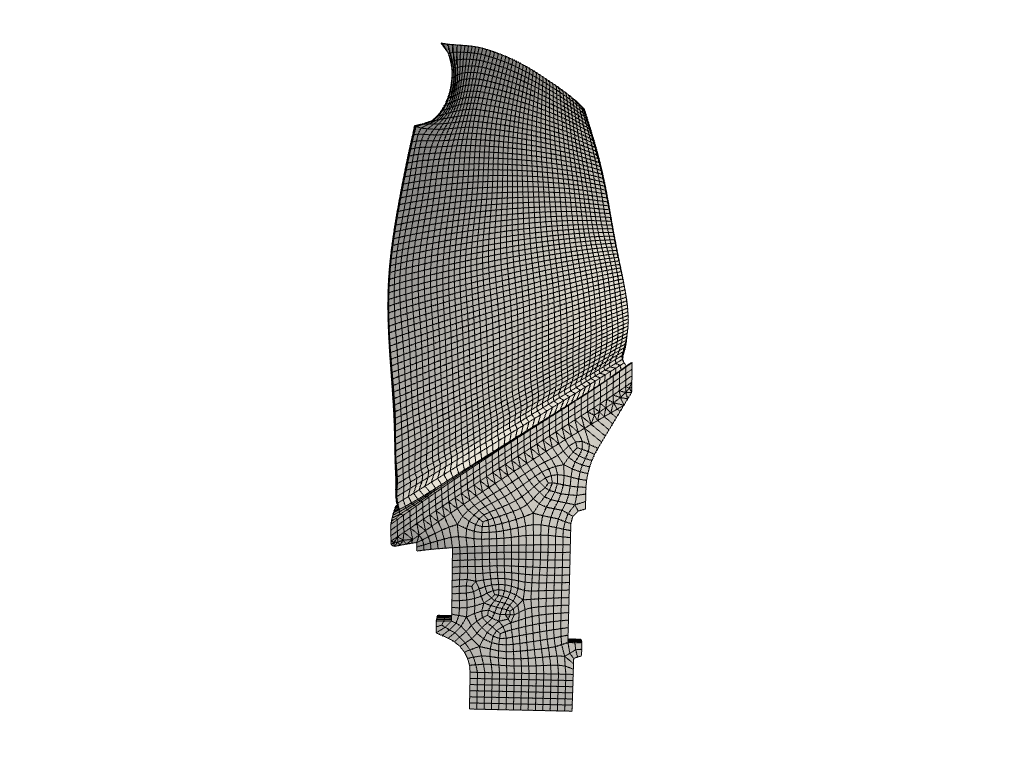
\includegraphics[height=1.0cm, , trim={13cm, 7cm, 13cm, 1cm}, clip]{./figures/pbs4_blend_12.png}};

    \node [block, below of=block1, yshift=-0.50cm] (block13) {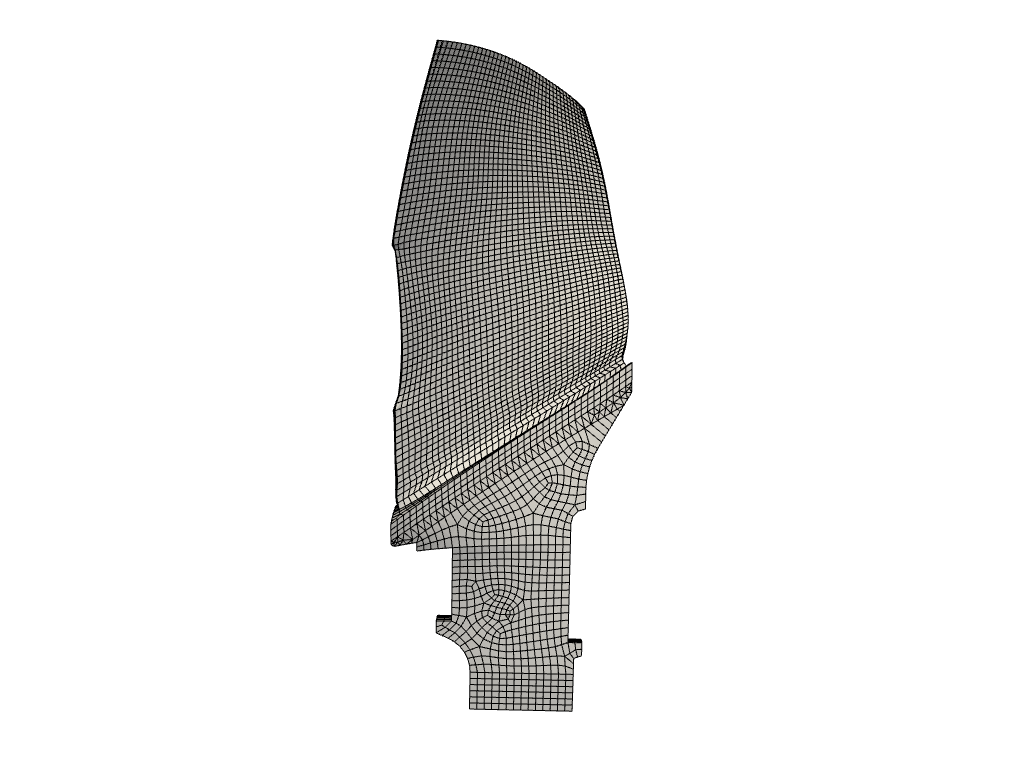
\includegraphics[height=1.0cm, , trim={13cm, 7cm, 13cm, 1cm}, clip]{./figures/pbs4_blend_13.png}};
    \node [block, below of=block2, yshift=-0.50cm] (block14) {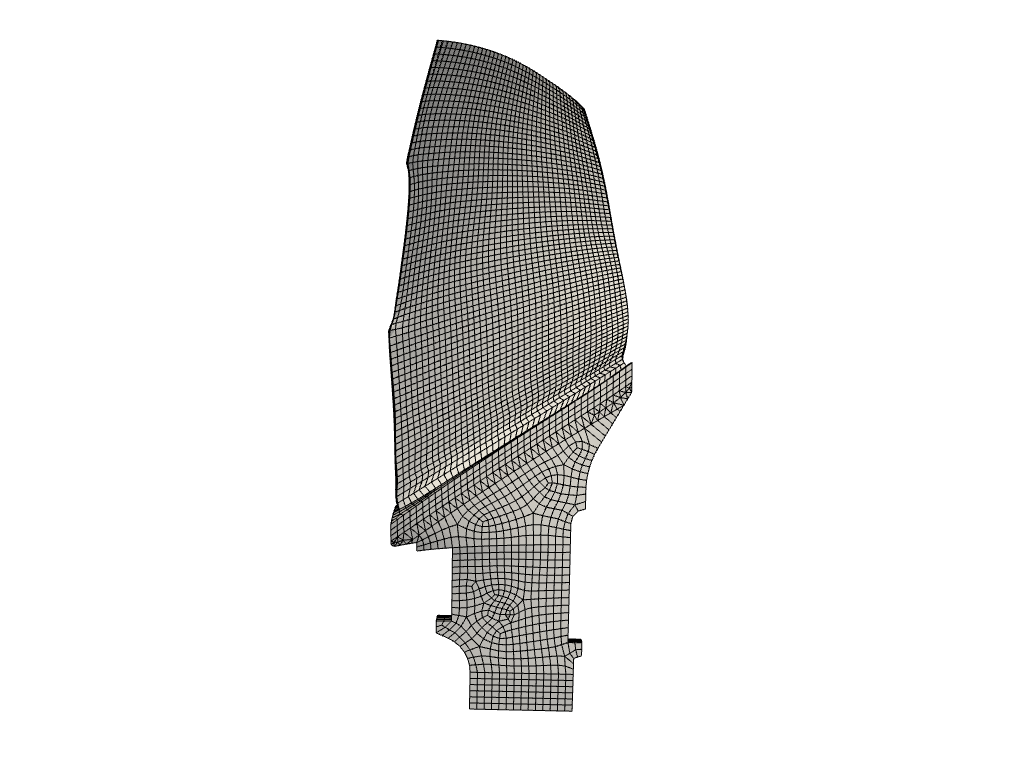
\includegraphics[height=1.0cm, , trim={13cm, 7cm, 13cm, 1cm}, clip]{./figures/pbs4_blend_14.png}};
    \node [block, below of=block3, yshift=-0.50cm] (block15) {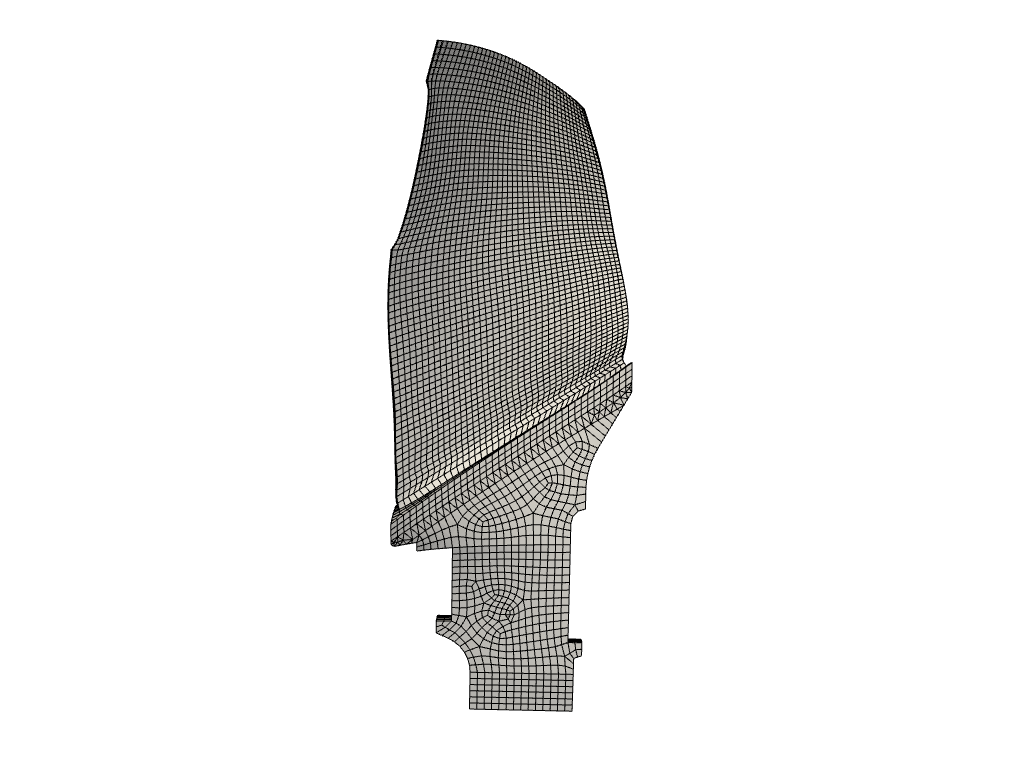
\includegraphics[height=1.0cm, , trim={13cm, 7cm, 13cm, 1cm}, clip]{./figures/pbs4_blend_15.png}};
    \node [block, below of=block4, yshift=-0.50cm] (block16) {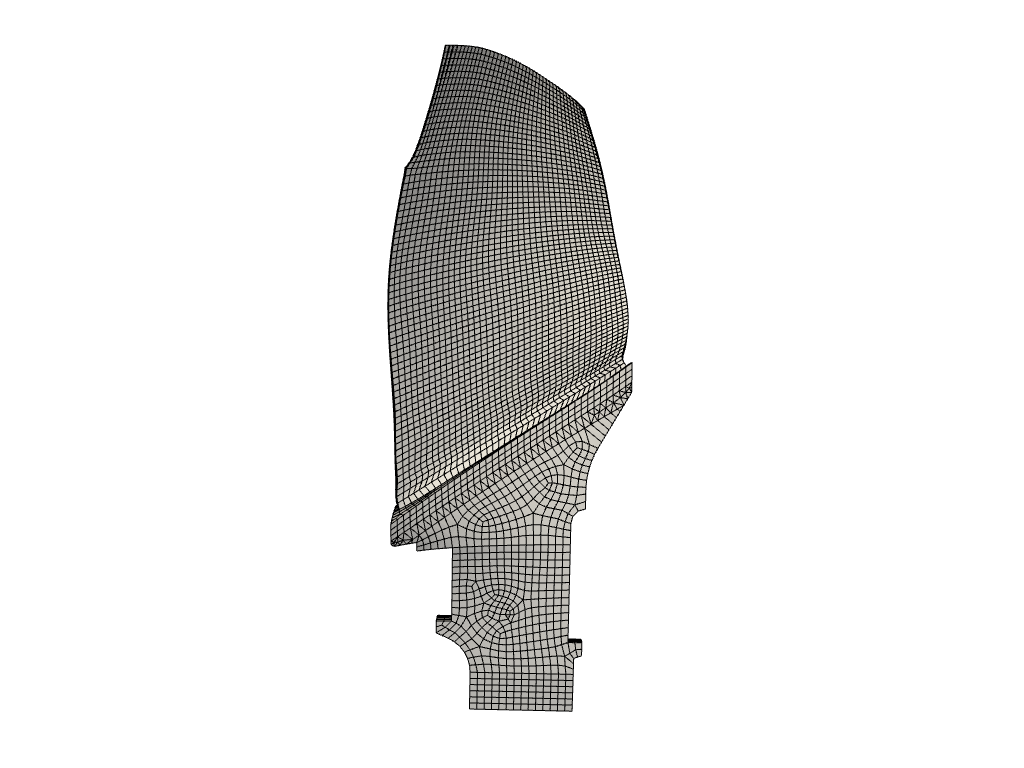
\includegraphics[height=1.0cm, , trim={13cm, 7cm, 13cm, 1cm}, clip]{./figures/pbs4_blend_16.png}};

    \node [block, below of=block13, yshift=-0.1cm] (block17) {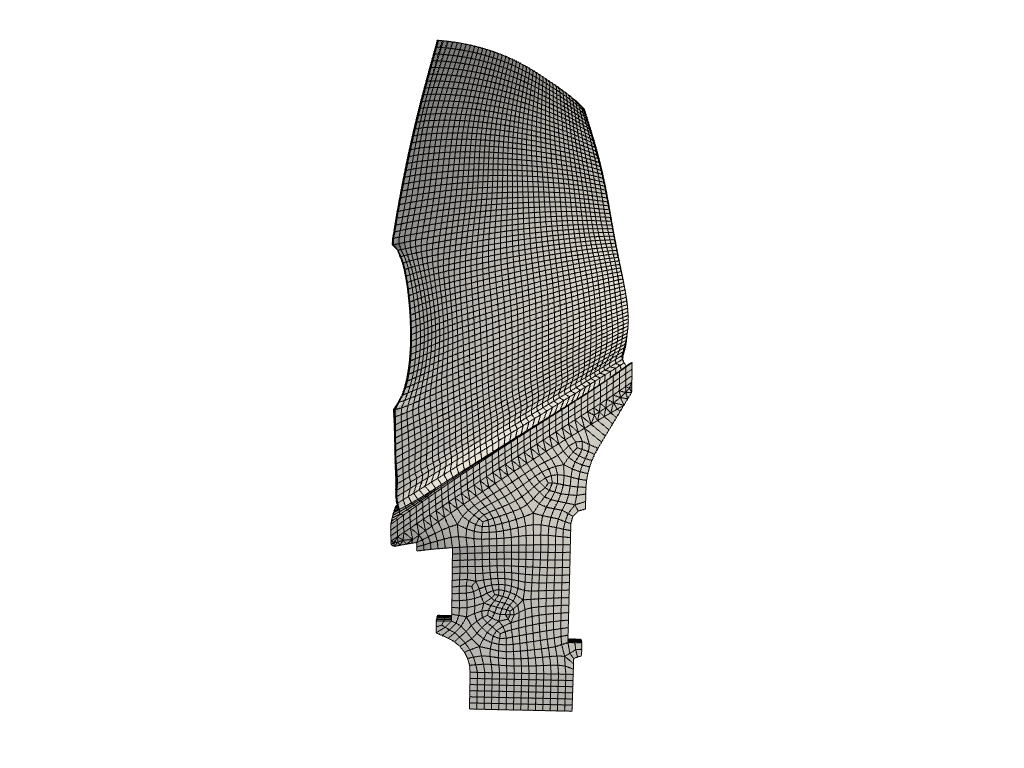
\includegraphics[height=1.0cm, , trim={13cm, 7cm, 13cm, 1cm}, clip]{./figures/pbs4_blend_17.png}};
    \node [block, below of=block14, yshift=-0.1cm] (block18) {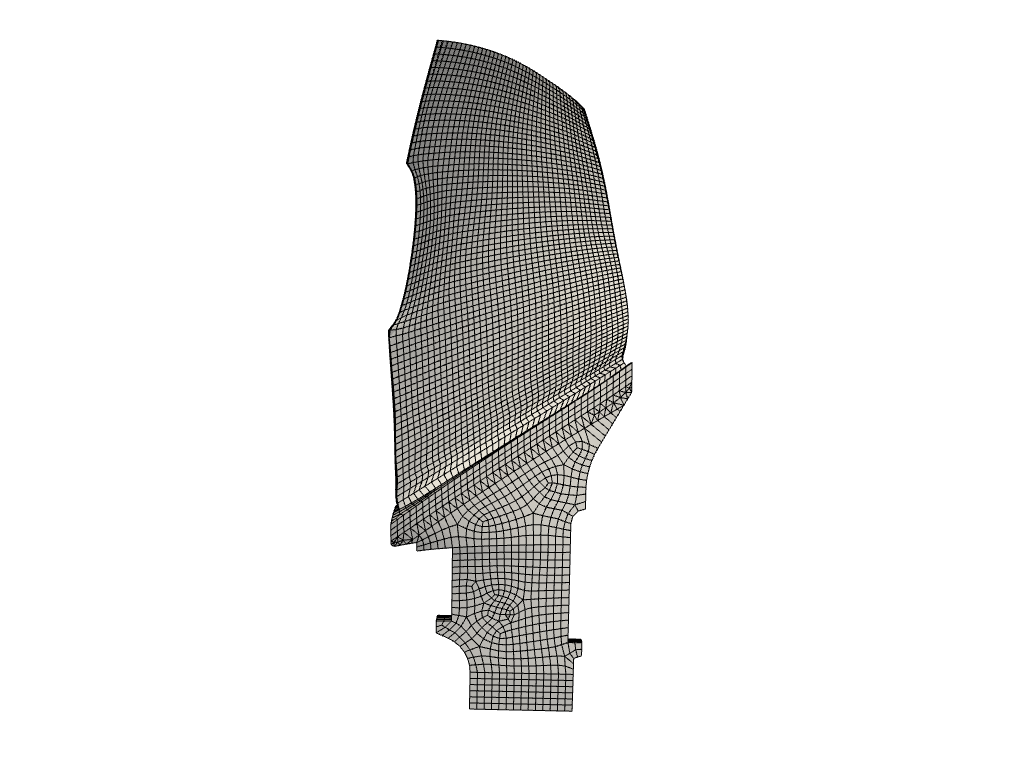
\includegraphics[height=1.0cm, , trim={13cm, 7cm, 13cm, 1cm}, clip]{./figures/pbs4_blend_18.png}};
    \node [block, below of=block15, yshift=-0.1cm] (block19) {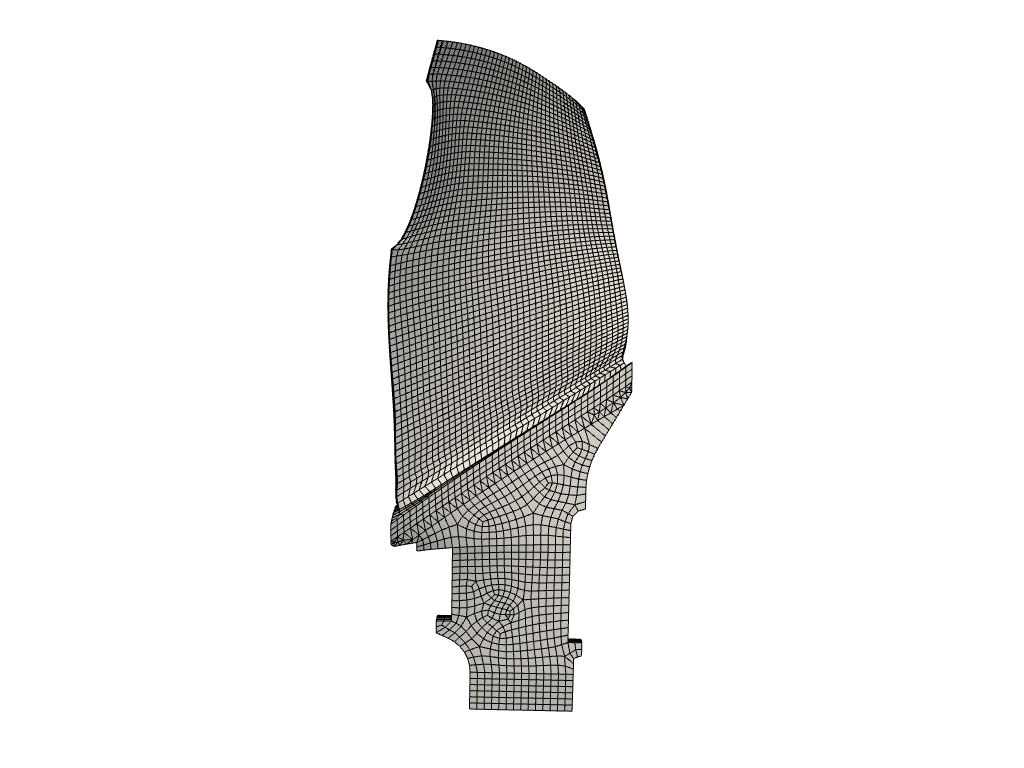
\includegraphics[height=1.0cm, , trim={13cm, 7cm, 13cm, 1cm}, clip]{./figures/pbs4_blend_19.png}};
    \node [block, below of=block16, yshift=-0.1cm] (block20) {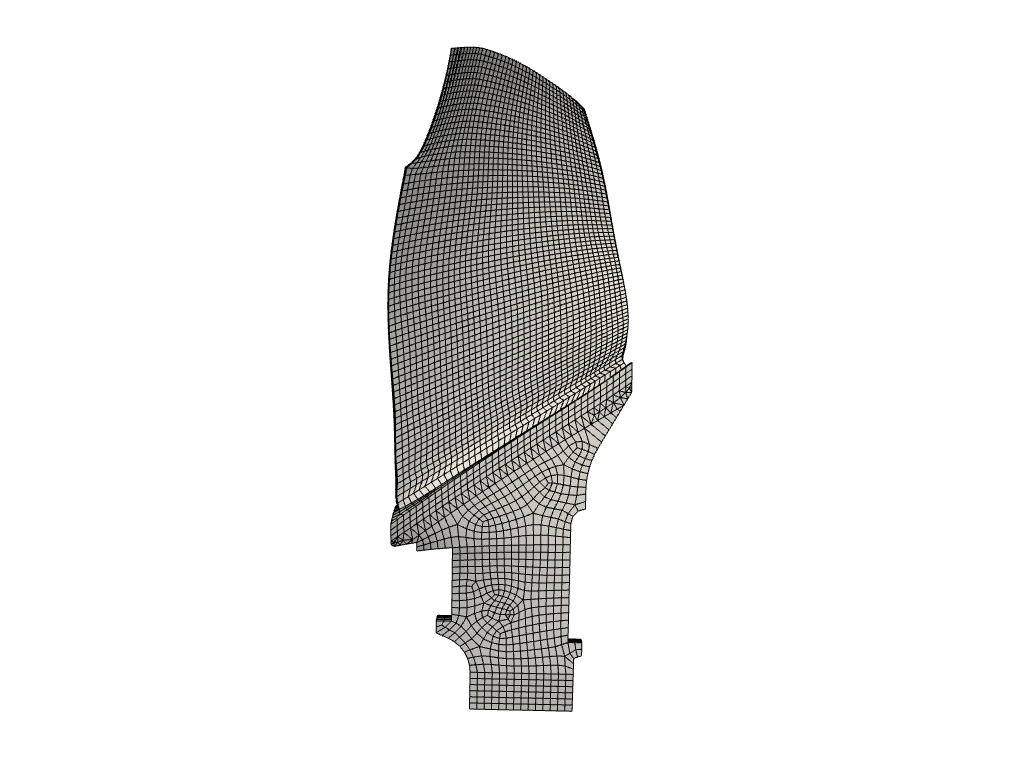
\includegraphics[height=1.0cm, , trim={13cm, 7cm, 13cm, 1cm}, clip]{./figures/pbs4_blend_20.png}};

    \node [block, below of=block17, yshift=-0.1cm] (block21) {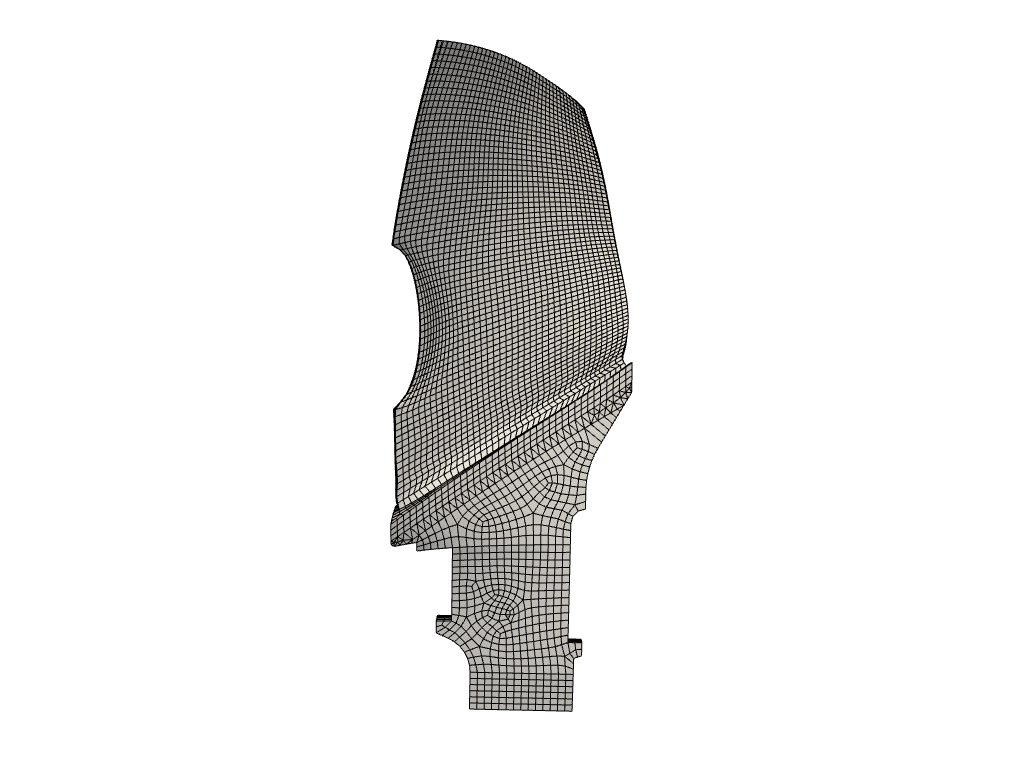
\includegraphics[height=1.0cm, , trim={13cm, 7cm, 13cm, 1cm}, clip]{./figures/pbs4_blend_21.png}};
    \node [block, below of=block18, yshift=-0.1cm] (block22) {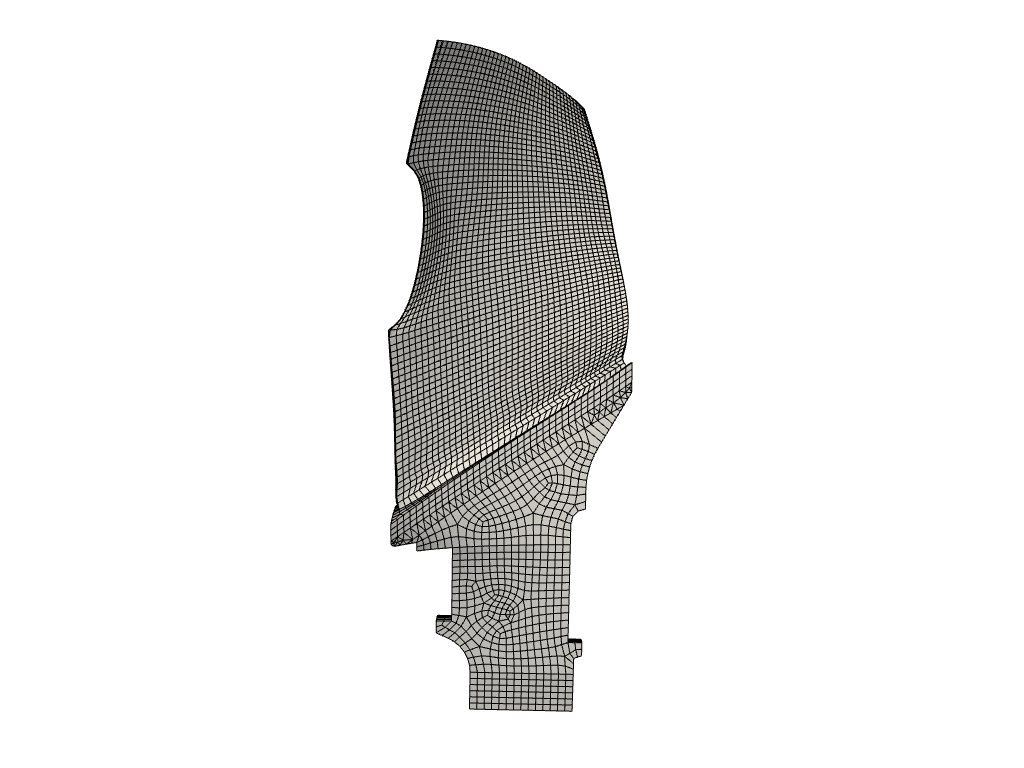
\includegraphics[height=1.0cm, , trim={13cm, 7cm, 13cm, 1cm}, clip]{./figures/pbs4_blend_22.png}};
    \node [block, below of=block19, yshift=-0.1cm] (block23) {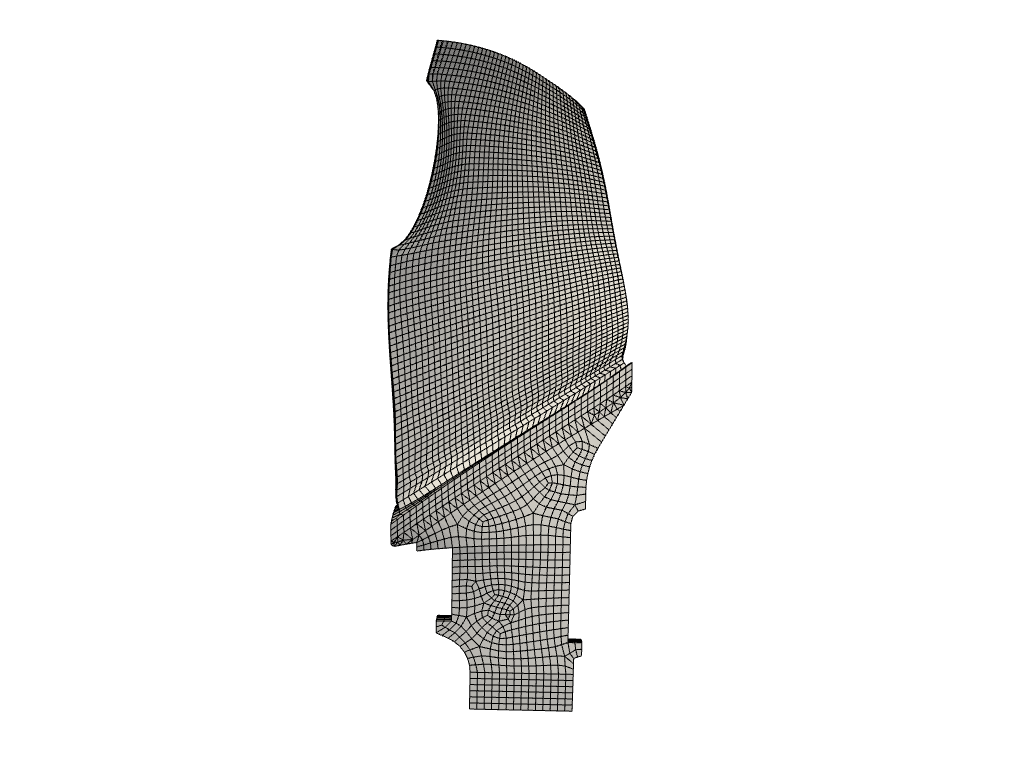
\includegraphics[height=1.0cm, , trim={13cm, 7cm, 13cm, 1cm}, clip]{./figures/pbs4_blend_23.png}};
    \node [block, below of=block20, yshift=-0.1cm] (block24) {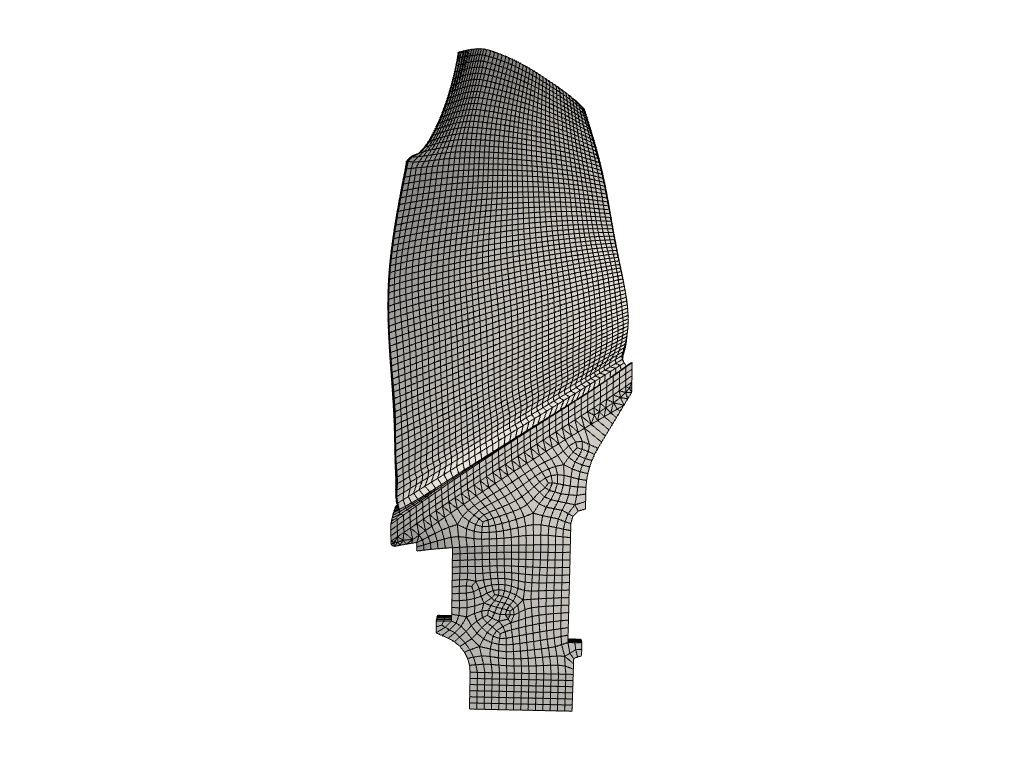
\includegraphics[height=1.0cm, , trim={13cm, 7cm, 13cm, 1cm}, clip]{./figures/pbs4_blend_24.png}};

    \node [] at (6.0,-0.75) {Span Location};
    \draw [->] (2.5, -0.75) -- (4.5, -0.75);
    \draw [->] (7.5, -0.75) -- (9.5, -0.75);

    \node [align=center] at (1.7, 1.1) {Blend\\ Depth};
    \draw [->] (1.7, 1.6) -- (1.7, 2.7);
    \draw [->] (1.7, -.4) -- (1.7, 0.6);
    \node [align=center] at (1.7, -2.6) {Blend\\ Depth};
    \draw [->] (1.7, -1.0) -- (1.7, -2.1);
    \draw [->] (1.7, -3.1) -- (1.7, -4.1);

    \draw [decorate,decoration={brace,amplitude=10pt,mirror,raise=4pt},yshift=0pt]
    (9.55, -0.4) -- (9.55, 2.7) node [black, midway, xshift=0.95cm, align=center] {Aspect\\ Ratio\\ A};

    \draw [decorate,decoration={brace,amplitude=10pt,mirror,raise=4pt},yshift=0pt]
    (9.55, -4.1) -- (9.55, -1.0) node [black, midway, xshift=0.95cm, align=center] {Aspect\\ Ratio\\ B};

    %\path [line] (init) |- (block5);
    \end{tikzpicture}
  
\end{frame}

%-------------------------------------------------------------------------------------------------------#
\begin{frame}
  \frametitle{Design with AFRL Morph X}
  \framesubtitle{Simplify Hex Mesh Generation - Morph defeatured FEM to Complex Surface}

  \begin{center}
    \begin{tikzpicture}
      \node (img1) {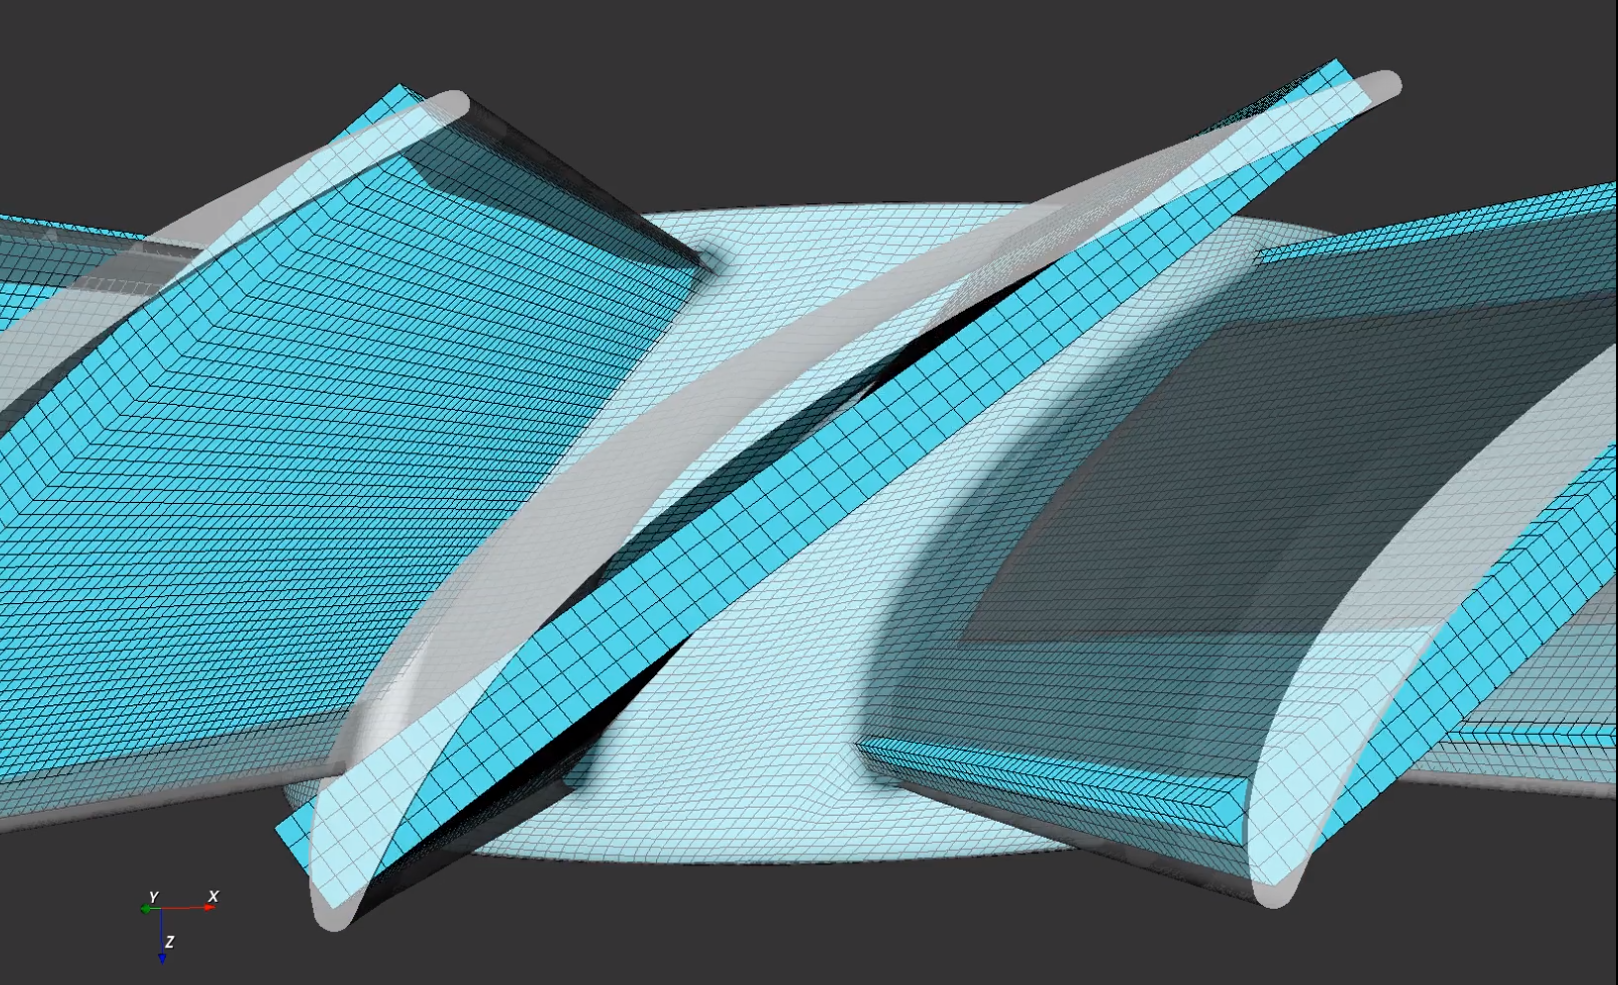
\includegraphics[height=3cm]{./figures/cant1.png}};
      %%\pause
      \node (img2) at (img1.south east) [yshift=-0.25cm]{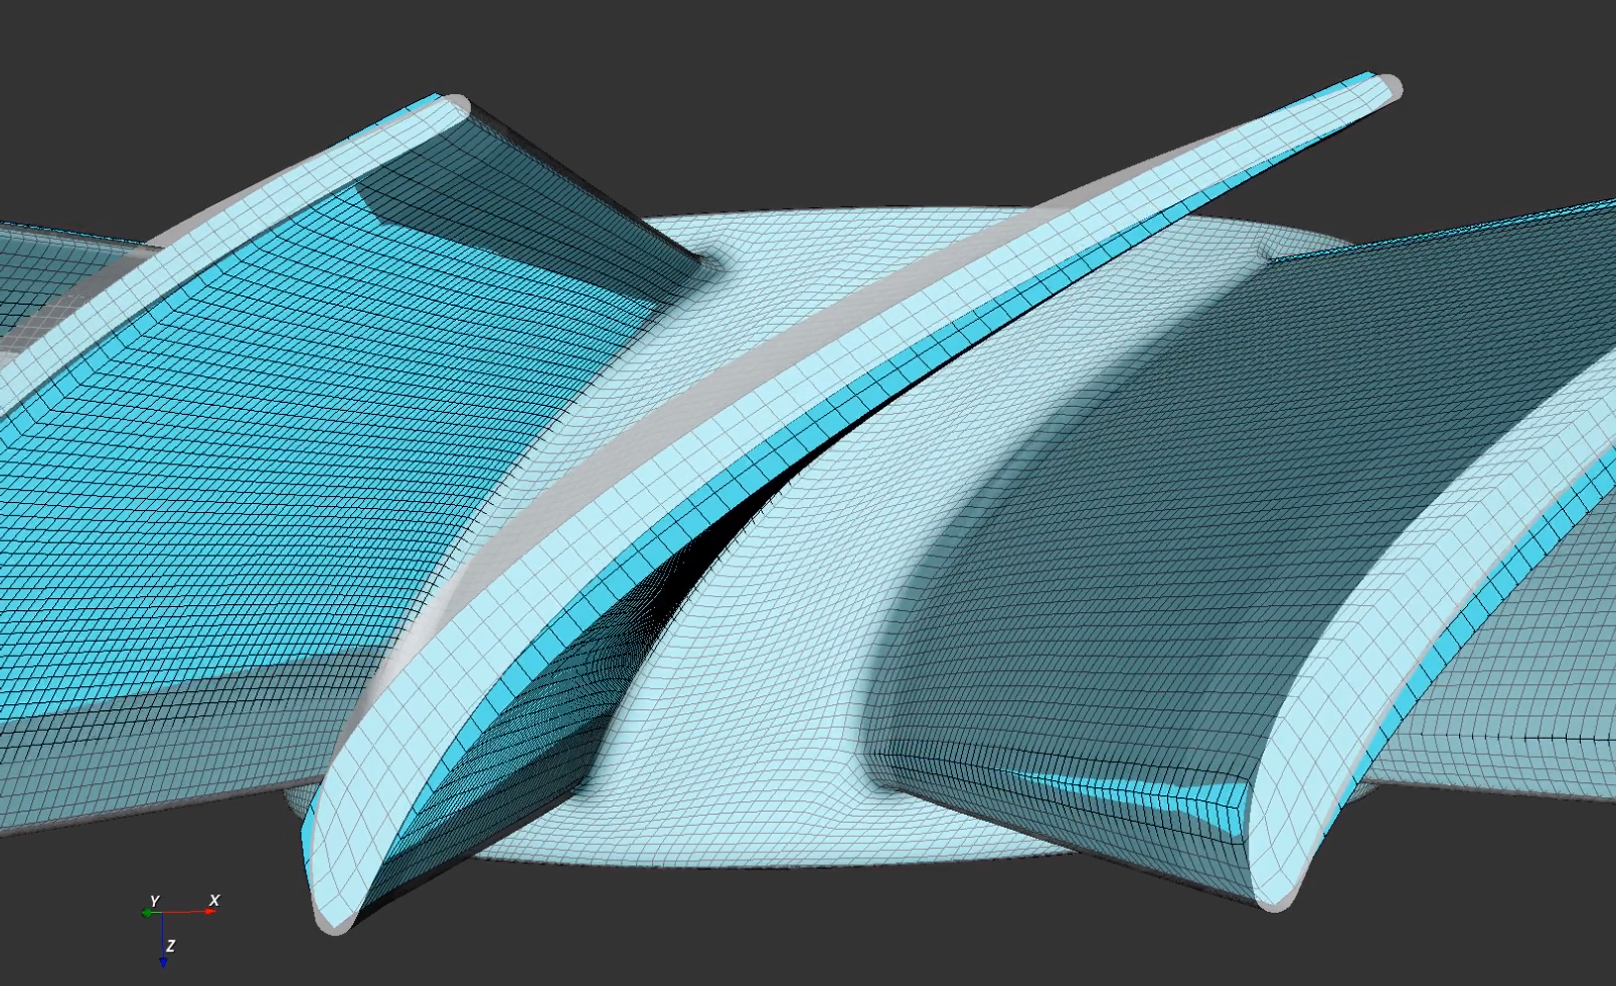
\includegraphics[height=3cm]{./figures/cant2.png}};
      %%\pause
      \node (img3) at (img2.south east) [yshift=-0.25cm] {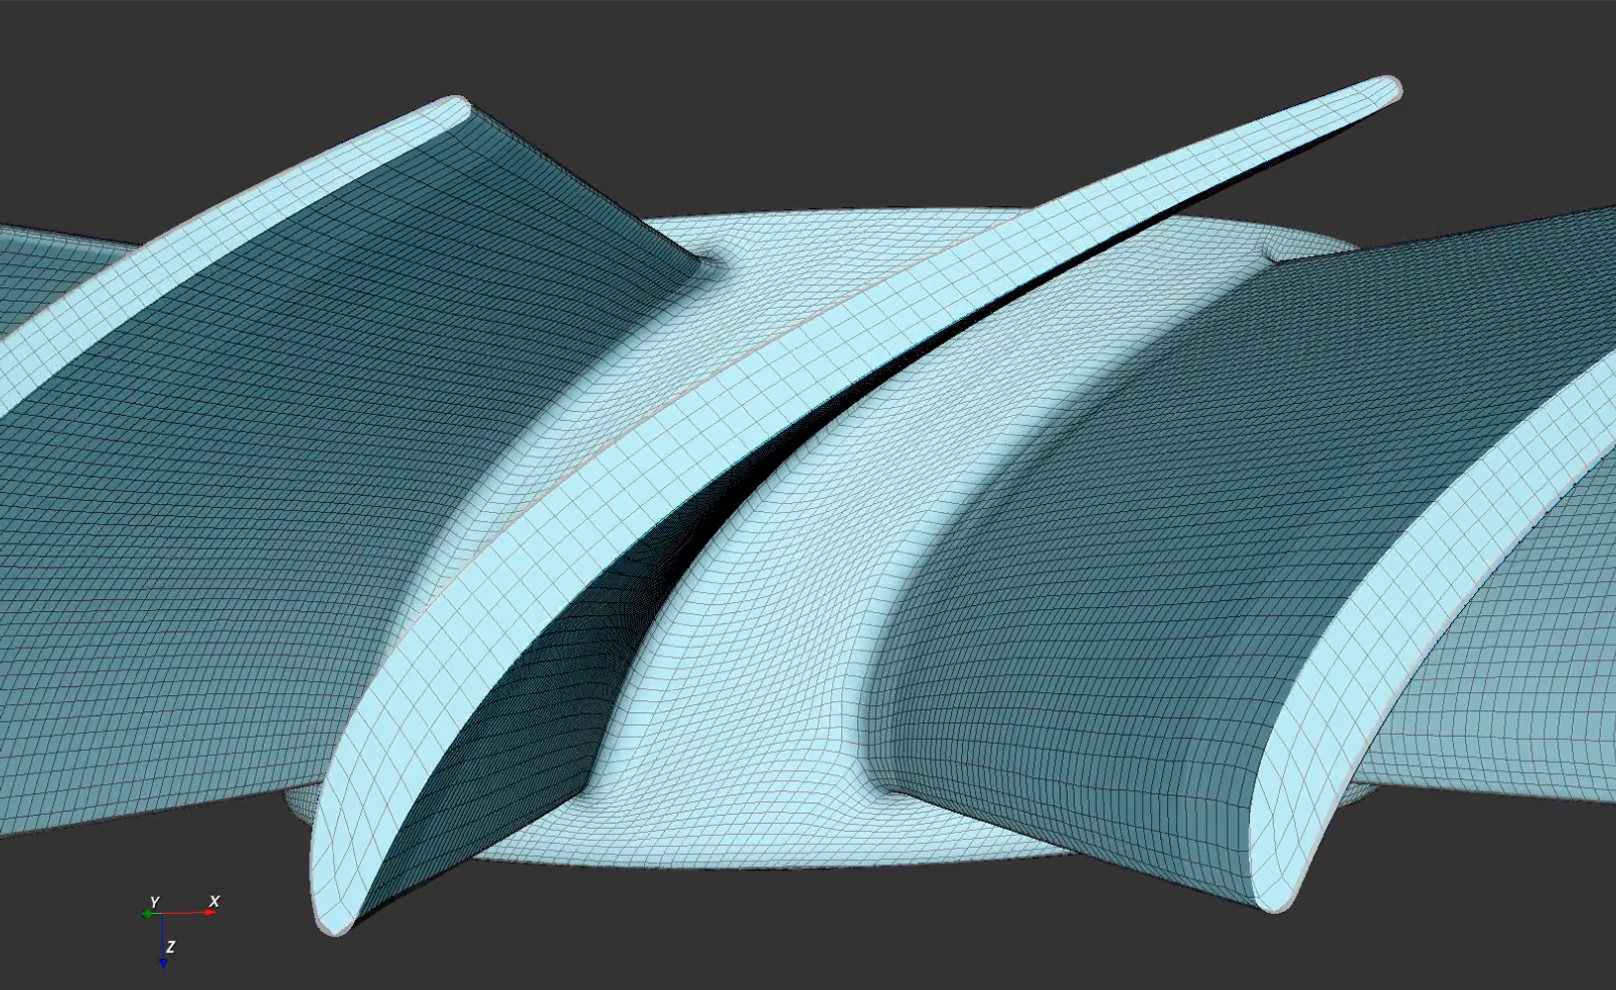
\includegraphics[height=3cm]{./figures/cant3.png}};
    \end{tikzpicture}
  \end{center}
\end{frame}

%-------------------------------------------------------------------------------------------------------#
\begin{frame}
  \frametitle{Animation - Click image to Play}
  %%\framesubtitle{Morph Simple Plate FEM to Complex 3D Turbine Airfoil Surface}

  \begin{figure}
    \centering    
    \movie[label=show3, width=1.0\textwidth, poster, autostart, showcontrols, loop]{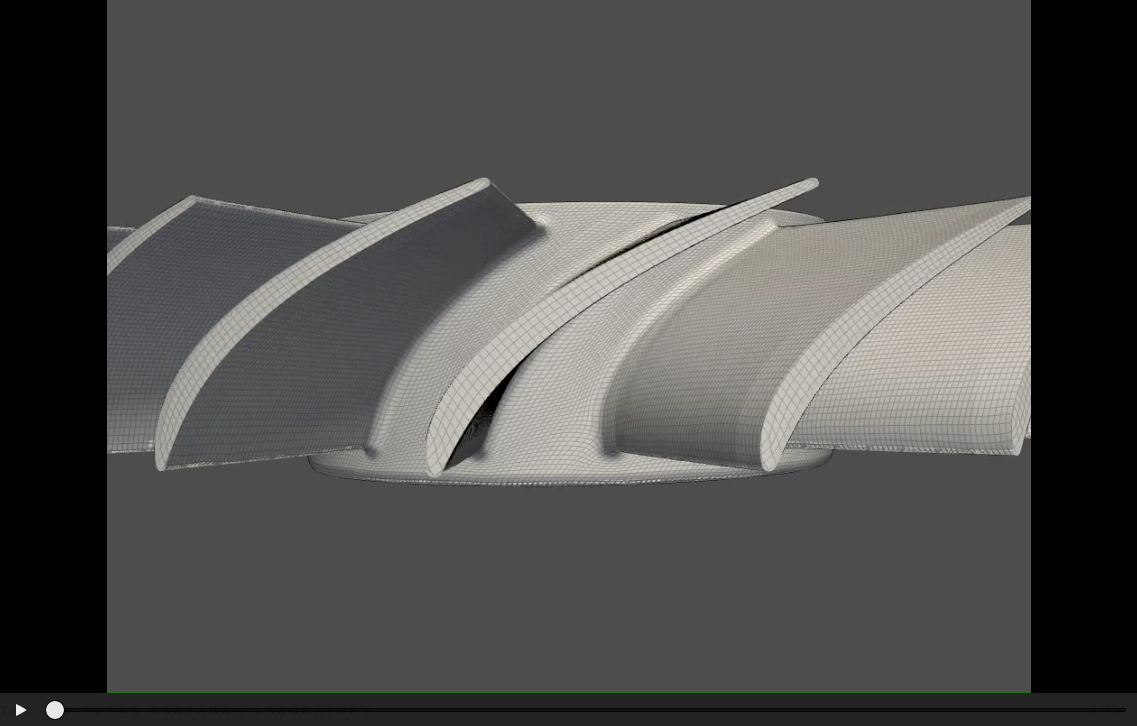
\includegraphics[width=1.0\textwidth]{./figures/jetcat_vidcover.png}}{./figures/jetcat_simvid.mp4}
 \end{figure} 
\end{frame}

%-------------------------------------------------------------------------------------------------------#
\begin{frame}
  \frametitle{Manufacturing with AFRL Morph X}
  \framesubtitle{It starts with measuring variation of a real part and comparing to Design Intent}
  %% \vspace{-2.5mm}

  \begin{tikzpicture}
    \node (img0) at (0, 0) [label=below:Geometry Measurement, inner sep=-2pt] {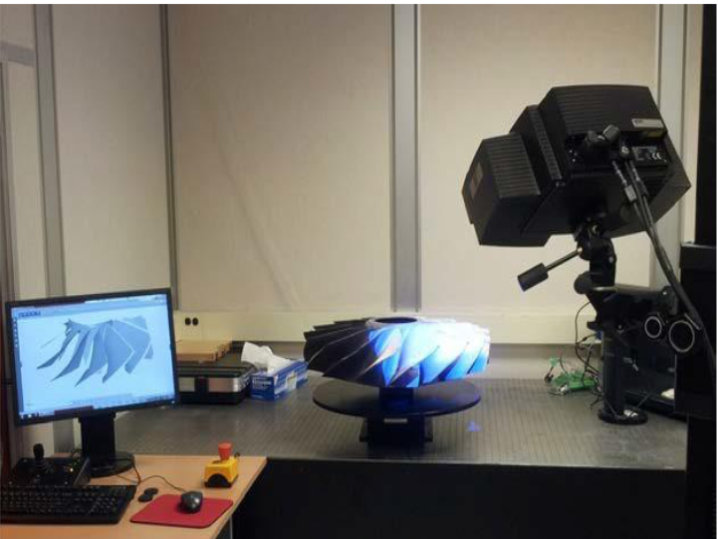
\includegraphics[height=2.5cm]{./figures/adlarfatos.png}};
    \node (img0b) at (img0.south) [label=below:FEM Software, yshift=-2.3cm, inner sep=-2pt] {
\includegraphics[height=2.5cm]{./figures/ansys.png}};
    \node (img1) at (img0.east) [label={[align=center, below, yshift=-2.25cm]STL Surface}, xshift=2.5cm, inner sep=-9pt] {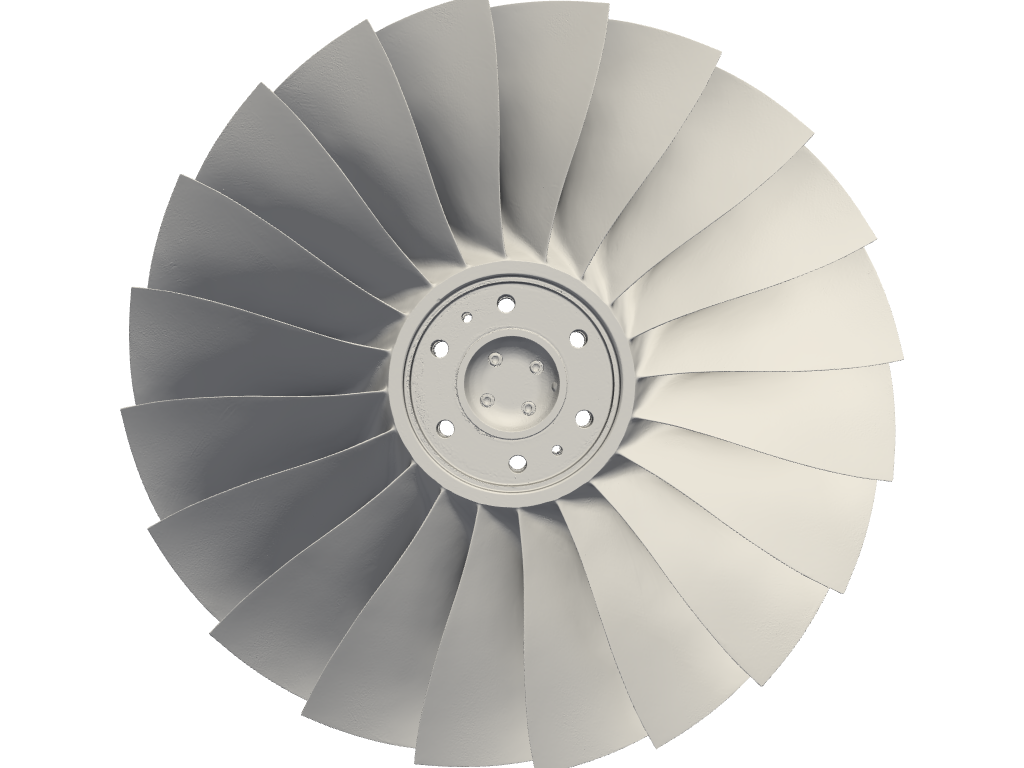
\includegraphics[height=2.5cm]{./figures/pbs_surf.png}};
    \node (img2) at (img1.south) [label={[align=center, below, yshift=-2.25cm]Design FEM}, yshift=-2.5cm, inner sep=-9pt]{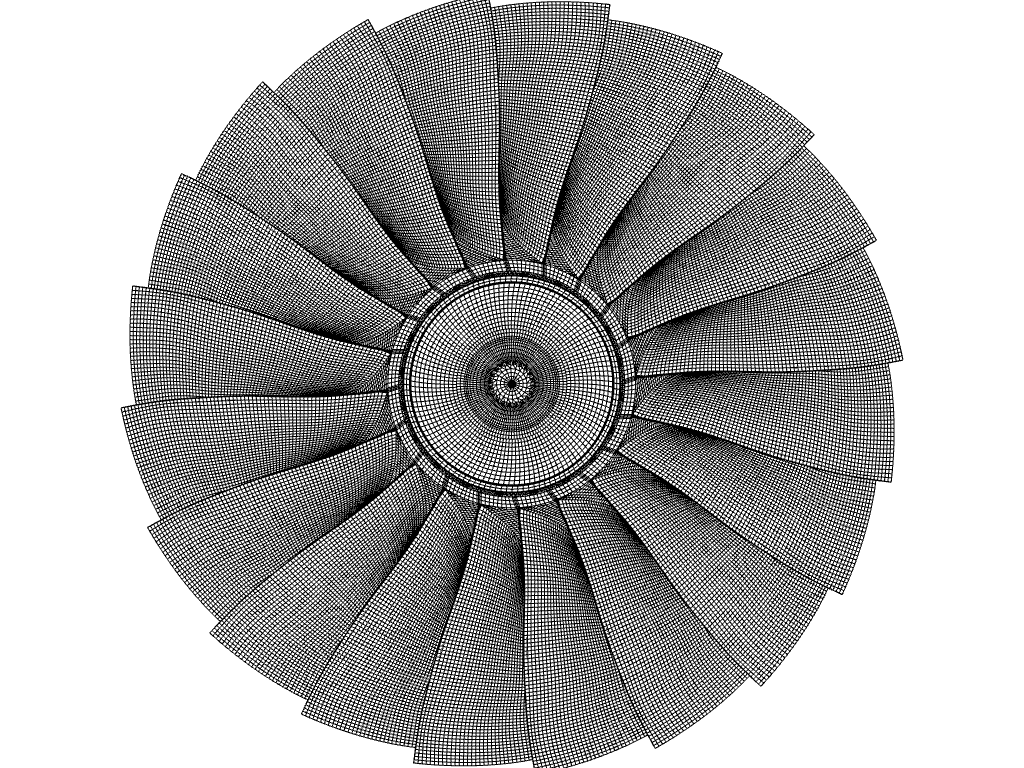
\includegraphics[height=2.5cm]{./figures/pbs_fem.png}};
    \node (img3) at (img1.south east) [label={[align=center, above, yshift=0.25cm]Manufacturing\\ Deviations}, yshift=-0.8cm, xshift=2.0cm, inner sep=-7pt] {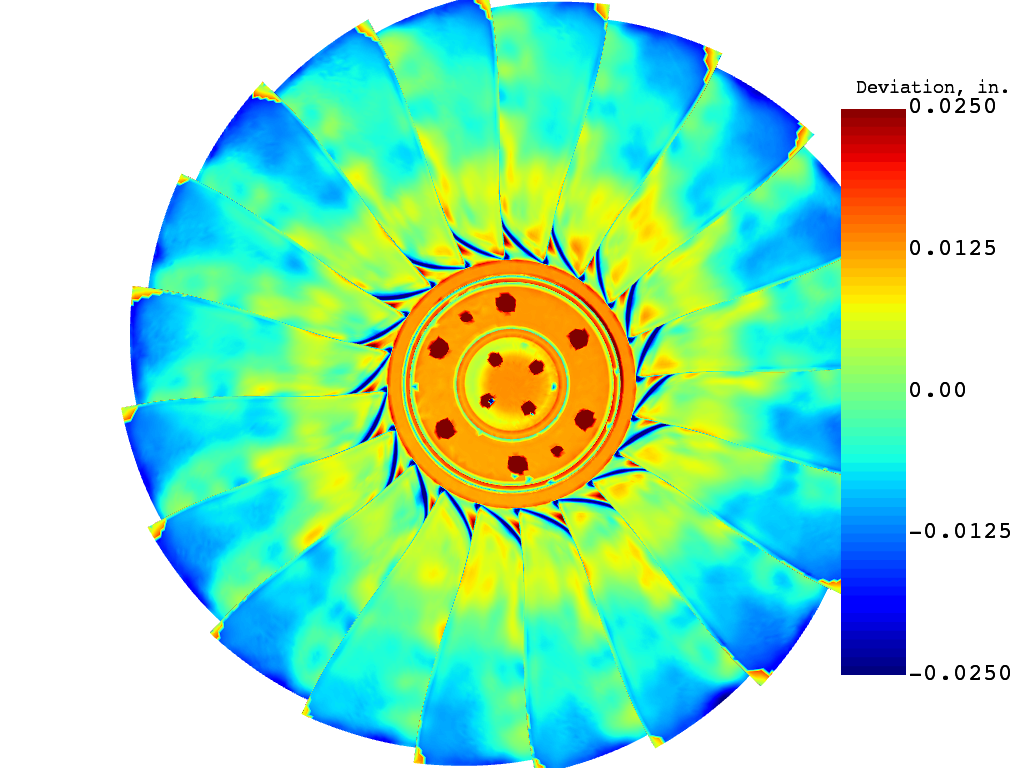
\includegraphics[height=3.0cm]{./figures/pbs_deviation.png}};

    \draw[->,thick] (img0.east) -- (img1.west);
    \draw[->,thick] (img0b.east) -- (img2.west);
    \draw[->,thick] (img1.south east) -- (img3.west);
    \draw[->,thick] (img2.north east) -- (img3.west);
    
    \end{tikzpicture}

\end{frame}
%-------------------------------------------------------------------------------------------------------#
\begin{frame}
  \frametitle{Manufacturing with AFRL Morph X}
  \framesubtitle{AFRL Morph X updates the Design FEM to match the STL surface within 0.001''}
  \begin{tikzpicture}
    \node (img1) at (0, 0) [label={[align=center, below, yshift=-2.5cm]STL Surface}, yshift=-.5cm, xshift=0cm, inner sep=-2pt] {\includegraphics[height=2.5cm]{./figures/pbs_surf.png}};
    \node (img2) at (img1.south) [label={[align=center, below, yshift=-2.5cm]Design FEM}, yshift=-2.65cm, inner sep=-2pt]{\includegraphics[height=2.5cm]{./figures/pbs_fem.png}};
    \node [draw] at (3.5, -2.4) (circle) {\includegraphics[height=2.5cm]{./figures/morph_logo.png}};
    \node (img3) at (circle.east) [label={[align=center, above, yshift=0.5cm]Morphed FEM\\ Deviations from STL}, xshift=2.5cm, inner sep=-9pt]{\includegraphics[height=3.0cm]{./figures/pbs_morphdev.png}};

    \draw[->,thick] (img1.east) -| (circle.north);
    \draw[->,thick] (img2.east) -| (circle.south);
    \draw[->,thick] (circle.east) -- (img3.west);
  \end{tikzpicture}

\end{frame}
%-------------------------------------------------------------------------------------------------------#
\begin{frame}
  \frametitle{Manufacturing with AFRL Morph X}
  \framesubtitle{Morphed FEM is a Computational Replica of Physical Part}
  \begin{tikzpicture}
    \node (img3) at (0, 0) [label={[align=center, above, yshift=-3.75cm]Morphed FEM\\ Computational Replica}, xshift=0.0cm, inner sep=-9pt]{\includegraphics[height=3.0cm]{./figures/pbs_morphdev.png}};
    \node (img4) at (img3.east) [label=below:FEM Software, xshift=2.25cm, inner sep=-2pt] {\includegraphics[height=2.5cm]{./figures/ansys.png}};
    \node (img5) at (img4.north east) [label={[align=center, below, yshift=-2.5cm]Blade to Blade\\Variation}, xshift=2.5cm]{\includegraphics[height=2.5cm]{./figures/b2b_scatter_m5}};
    \node (img6) at (img5.south) [label={[align=center, below, yshift=-2.5cm]Rotor to Rotor\\Variation}, yshift=-2.0cm]{\includegraphics[height=2.5cm]{./figures/mode_freq_all.pdf}};
    \draw[->,thick] (img3.east) -- (img4.west);
    \draw[->,thick] (img4.east) -- (img5.west);
    \draw[->,thick] (img4.east) -- (img6.west);
  \end{tikzpicture}

\end{frame}

%-------------------------------------------------------------------------------------------------------#
\begin{frame}
  \frametitle{Animation - Click image to Play}
  %%\framesubtitle{Morph Simple Plate FEM to Complex 3D Turbine Airfoil Surface}

  \begin{figure}
    \centering    
    \movie[label=show3, width=1.0\textwidth, poster, autostart, showcontrols, loop]{\includegraphics[width=1.0\textwidth]{./figures/pbs_vidcover.png}}{./figures/pbs_morphvid_align.mp4}
 \end{figure} 
\end{frame}

%-------------------------------------------------------------------------------------------------------#
\begin{frame}
  \frametitle{Operations with AFRL Morph X}
  \framesubtitle{Integrating with Maintenance, Repair, and Operations with Morph X}
    \begin{tikzpicture}
      \node (img0) at (0, 0) [yshift=-3.5cm, xshift=0.0cm, inner sep=0pt]{\includegraphics[height=3.0cm]{./figures/depot_mx.jpeg}};
      % \node (img1) at (img0.east) [label={[align=center, above, yshift=-3.0cm]Airfoil Leading Edge Blend Repair}, xshift=3.4cm, inner sep=-2pt]{\includegraphics[height=2.5cm]{./figures/pbs4_sector_1_blend_3.png}};
      \node (img1) at (img0.east) [label={[align=center, above, yshift=-3.0cm]Airfoil Leading Edge Blend Repair}, xshift=3.4cm, inner sep=-2pt]{\includegraphics[trim={0.5cm 0 0.5cm 0}, clip, height=2.5cm]{./figures/pbs4_unblend.png}};
      \node (img1a) at (img0.east) [xshift=4.8cm, inner sep=-2pt]{\includegraphics[trim={12.0cm 0 12.0cm 0}, clip, height=2.5cm]{./figures/pbs4_blend.png}};
      \node (img1b) at (img0.east) [xshift=2.0cm, inner sep=-2pt]{\includegraphics[trim={12.0cm 0 12.0cm 0}, clip, height=2.5cm]{./figures/pbs4_blend_clip.png}};
      \node (img2) at (img0.south) [label={[align=center, above, yshift=-3.0cm] Assess Damage}, yshift=-2.0cm, inner sep=-2pt]{\includegraphics[height=2.5cm]{./figures/mrb_pic.png}};
      \node (img3) at (img1.south) [label={[align=center, above, yshift=-3.0cm] Safety Review  Board}, yshift=-2.4cm, inner sep=-2pt]{\includegraphics[height=2.5cm]{./figures/safety_pic.png}};
    \end{tikzpicture}
\end{frame}
%-------------------------------------------------------------------------------------------------------#

\begin{frame}
  \frametitle{More with AFRL Morph X}
  \framesubtitle{}

  \begin{tikzpicture}
    \node (img0) at (0, 0) [yshift=-3.5cm, xshift=0.0cm, inner sep=0pt]{\includegraphics[height=2.0cm]{./figures/hptmoviecrop.png}};
    \node (img1) at (img0.south east) [label={[align=center, above, xshift=-0.75cm, yshift=-2.5cm]Turbine CFD Mesh Morphing}, yshift=-0.5cm, xshift=0.0cm, inner sep=0pt]{\includegraphics[height=2.0cm]{./figures/EfficiencyHistogram.pdf}};
    \node (img2) at (img0.east) [label={[align=center, below, yshift=-3.0cm] First Article Analysis}, yshift=-0.5cm, xshift=5.0cm, inner sep=-2pt]{\includegraphics[trim={0.0cm 0 0.0cm 0}, clip, height=3.0cm]{./figures/PTR_point_cloud.png}};
    \node (img3) at (img0.south) [label={[align=center, below, yshift=-2.5cm] ML/AI Training Data Generator}, xshift=0.5cm, yshift=-3.25cm, inner sep=-2pt]{\includegraphics[trim={0cm 0 0.0cm 0}, clip, height=2.5cm]{./figures/pbs4_gspfreq_m6.png}};
    \node (img4) at (img2.south) [label={[align=center, below, yshift=-2.5cm] Additive Part Models}, xshift=0.0cm, yshift=-2.4cm, inner sep=-2pt]{\includegraphics[trim={0cm 0 0.0cm 0}, clip, height=2.5cm]{./figures/jcturb_morph_sn.png}}; 
  \end{tikzpicture}
\end{frame}
%-------------------------------------------------------------------------------------------------------#
 \begin{frame}
  \frametitle{Even more with AFRL Morph X}
  \framesubtitle{}

  \begin{tikzpicture}
    \node (img0) at (0, 0) [label={[align=center, below, xshift=-0.0cm, yshift=-3.0cm]CMM Data Capable}, yshift=-3.5cm, xshift=0.0cm, inner sep=0pt]{\includegraphics[height=3.0cm]{./figures/cmm_points.png}};
    \node (img1) at (img0.east) [label={[align=center, below, xshift=0.0cm, yshift=-3.0cm]Improved Instrumentation}, yshift=0.0cm, xshift=3.5cm, inner sep=0pt]{\includegraphics[height=3.0cm]{./figures/strain_gage.png}};
    \node (img2) at (img0.south) [label={[align=center, below, yshift=-3.0cm]Improved Model Validation}, yshift=-2.0cm, xshift=0.0cm, inner sep=-2pt]{\includegraphics[trim={0.0cm 0 0.0cm 0}, clip, height=3.0cm]{./figures/pbs_rig.png}};
    \node (img3) at (img2.east) [label={[align=center, below, yshift=-2.5cm]Adaptive Toolpath Generation}, xshift=3.5cm, yshift=0.0cm, inner sep=-2pt]{\includegraphics[trim={0cm 0 0.0cm 0}, clip, height=2.5cm]{./figures/blade_optomec_xsec.png}};
  \end{tikzpicture}

  %% Morph any surface to another.

\end{frame}
 %-------------------------------------------------------------------------------------------------------#
\begin{frame}
  \frametitle{AFRL Design X Interface}
  \framesubtitle{Scriptable for integration in automated workflows and GUI for user experience}

 \begin{columns}
    \begin{column}{0.5\textwidth}
      
        \begin{figure}
          \includegraphics[height=1.5in]{./figures/script.png}
          
        \end{figure}

    \end{column}
    \begin{column}{0.5\textwidth}

      \begin{figure}
       \includegraphics[height=1.25in]{./figures/GUI.png}
      \end{figure}
      
    \end{column}
  \end{columns}

\end{frame}
 
%-------------------------------------------------------------------------------------------------------#
\begin{frame}
  \frametitle{AFRL Design X Background}
  \framesubtitle{}

  \begin{itemize}
  \item Developed in Python, C, and C++ for 8+ years
  \item Accessible through GUI and Python API, Linux, Windows, and Mac OS
  \item Beta tested by Pratt \& Whitney for two years
  \item Operating in year 4 of 10 year non-exclusive license with Pratt \& Whitney
  \item P\&W provides licensing fees for use and support
  \item Utilized by large P\&W user base for wide range of applications
  \item Applied pervasively in AFRL research activities
  \end{itemize}

\end{frame}

%-------------------------------------------------------------------------------------------------------#

\begin{frame}
  \frametitle{AFRL Design X Background}
  \framesubtitle{Software Development}

  \begin{itemize}
  \item Software tested rigorously in continuous development and deployment (CI/CD) pipelines
  \item Leverages automated testing in a secure environment
  \item Enables high code coverage and stability testing through regression testing.
  \end{itemize}

      \begin{figure}
       \includegraphics[height=1.65in]{./figures/ci-trigger.png}
      \end{figure}

\end{frame}


%-------------------------------------------------------------------------------------------------------#

\begin{frame}
  \frametitle{AFRL Design X Background}
  \framesubtitle{Software Testing}

  \begin{itemize}
  \item AFRL Design X follows standard software development practices.
  \item Unit and regression tests ensure new features are added without breaking existing ones.
  \item Code coverage of $\geq$ 95\% required for all modules, and $\geq$ 98\% for core modules
  \end{itemize}

      \begin{figure}
       \includegraphics[height=1.65in]{./figures/pytest.png}
      \end{figure}

\end{frame}


%% %-------------------------------------------------------------------------------------------------------#

\begin{frame}
  \frametitle{AFRL Design X Background}
  \framesubtitle{Software Design: Modularity}

  \vspace{-5mm}
  \begin{columns}

    \begin{column}{0.6\textwidth}
      \begin{itemize}
      \item Software is a non-monolithic, modular, and composed of several packages.  Includes both GUI and batch packages.
      \item Designed to be expandable, adaptive, and compatible with modern Python 3.6 - 3.8 environments on Windows, Mac, and Linux.
      \item Installable from \textit{pip} via offline wheelhouse from GitHub releases.
      \item Compatible with standalone virtual environments, Jupyterlab webpages, or standard Python.
      \end{itemize}
    \end{column}

    \begin{column}{0.4\textwidth}
      \vspace{-1.0mm}
      \begin{figure}
        \includegraphics[height=2.5in]{./figures/packages_azure_light.png}
      \end{figure}
    \end{column}

\end{columns}


\end{frame}


%-------------------------------------------------------------------------------------------------------#
\frame{
  \frametitle{Closing Remarks}
  \begin{itemize}
  \item AFRL MORPH X adds value across the life cycle, from design, to manufacture, and through operations
  \item Rigorous software development practices have enabled rapid development and successful deployment 
  \item Windows demo software available and licensing opportunities
  \end{itemize}
}


\lastframe
    
\end{document}
